\section{Introduction}
\label{implementation_testing_introduction}

In this chapter we will present the results of the implementation and validation process used for developing the predictive model described in chapter \ref{chapter_theory_modelling}. Indeed, fundamental to our approach for approximating the latent motivational state of an individual is to have a model able to reliably predict the intensity of future behaviour (i.e. future engagement in a videogame context) given the history of interactions between an individual and a potential rewarding object (i.e. a videogame). To achieve this, we adopted a variation of bottom-up iterative model building \cite{gelman2020bayesian} in which first the simplest version of a model is designed, built and evaluated and then, based on perfromance and addition theoretical assumptions, a new improved version of the same model is proposed. At each stage of the process we evaluate the new version of the model against alternative approaches in order to test for hypotheses stated in the model design stage. Each section of this chapter corresponds to a different version of the model and will have the following structure. In \textbf{Model Design} we state the task the model is trying to solve, the design of such model and the theoretical assumptions that informed the design. In \textbf{Data} we describe the dataset used for evaluating the perfromance of our model along with any data-related processing. In \textbf{Model Comparison} we outline the alternative approaches against which the current model is compared and the various procedures and statistical analyses employed. In \textbf{Results} we report the outcomes of the model comparison procedure with particular focus on the assessment of the predictive accuracy. In \textbf{Model Criticism} we discuss what presented in the results section,in light of the theoretical assumptions used when designing the model, and highlight potential improvements to be carried out in the subsequent stage of the model building process.

\section{Joint Prediction of Long Term Behavioural Intensity}
\label{model_architecture_1}
In the first iteration of our model building process we focused on implementing and testing some of the core theoretical assumptions presented in chapter \ref{chapter_theory_modelling}, namely the importance of modelling temporal and non-linear dynamics in the interactions between an individual and a videogame. The experimental task used for this purpose aimed at predicting the long term intensity of interactions between an individual and a videogame given a set of behavioural metrics recorded during an initial observation period. Here, the observation period is defined as a small sequence of initial interactions between an individual and a videogame. In this specific context, we used churn and survival time as behavioural proxies for the expected intensity of future interactions. We briefly introduced these two concepts in section \ref{engagement_prediction}. More formally we can say that given a sequence of interactions with associated behavioural intensity $B_{t_1 : T}$, survival time is the amount of expected future playing activity at a given point $t_n$ \cite{ perianez2016churn, demediuk2018player, bertens2017games, kim2017churn, viljanen2018playtime}
\begin{equation}
\label{eq_survival}
    survival = \sum_{t_n}^{T}B_t
\end{equation}
while churn is the probability of observing a terminal event $C$ (usually formulated as a prolonged period of inactivity from the individual) after a given point $t_n$ \cite{hadiji2014predicting,runge2014churn, drachen2016rapid,milovsevic2017early, kim2017churn}.
\begin{equation}
\label{eq_churn}
    churn = \sum_{t_n}^{T}C_n = 1
\end{equation}
here the interactions going from $t_1: t_n$ define our observation period. It has to be noted that this task can be viewed as a special case of the more general formulation presented in section \ref{td_to_supervised} and correspond to predicting extinction and future ammount of sustained engagement after observing a handful of interactions following the point of engagement (according to O'Brien et al. \cite{o2008user} framework presented in section \ref{eng_reward_motivation}). Given this experimental context, the hypotheses that we wanted to evaluate in order to support our modelling intuitions were the following:
\begin{enumerate}
    \item Leveraging all the information present in the observation period is required for achieving higher predictive power.
    \item Approaches able to account for non-linear interactions in the considered behavioural metrics can outperform simpler additive models.
    \item The ability to model the type of sequential dynamics presented in section \ref{td_to_supervised} can have a positive effect on the predictive perfromance.
    \item It is possible to have a single model jointly predict the considered metrics of long term behavioural intensity without any loss of predictive accuracy.
    \item It is possible to have a single model performing the predictive task simultaneously across a wide range of games.
\end{enumerate}

\subsection{Model Design}
\label{model_design_1}
The first iteration of our ANN architecture, loosely inspired by the winning entry in \cite{lee2018game}, aims to jointly predict survival time and churn probability across a set of 6 different game contexts. This architecture, the `Bifurcating Model' (BM), is illustrated in Fig. \ref{fig: rnn_1}. 
\begin{figure}[ht]
\begin{center}
\begin{adjustbox}{width=0.7\textwidth}



\tikzset{every picture/.style={line width=0.75pt}} %set default line width to 0.75pt        

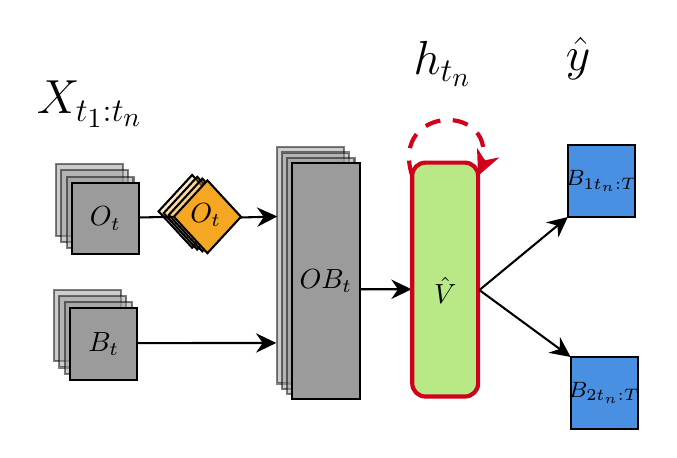
\begin{tikzpicture}[x=0.75pt,y=0.75pt,yscale=-1,xscale=1]
%uncomment if require: \path (0,300); %set diagram left start at 0, and has height of 300

%Shape: Diamond [id:dp06877884521197963] 
\draw  [fill={rgb, 255:red, 245; green, 166; blue, 35 }  ,fill opacity=0.25 ] (263.6,117.28) -- (279.77,134.81) -- (263.6,152.33) -- (247.43,134.81) -- cycle ;
%Shape: Diamond [id:dp5019197402707816] 
\draw  [fill={rgb, 255:red, 245; green, 166; blue, 35 }  ,fill opacity=0.25 ] (266.05,118.16) -- (282.22,135.68) -- (266.05,153.2) -- (249.89,135.68) -- cycle ;
%Shape: Diamond [id:dp6628494024847519] 
\draw  [fill={rgb, 255:red, 245; green, 166; blue, 35 }  ,fill opacity=0.25 ] (268.51,119.04) -- (284.68,136.56) -- (268.51,154.08) -- (252.34,136.56) -- cycle ;
%Shape: Rectangle [id:dp8304682723722553] 
\draw  [color={rgb, 255:red, 0; green, 0; blue, 0 }  ,draw opacity=0.5 ][fill={rgb, 255:red, 155; green, 155; blue, 155 }  ,fill opacity=0.5 ] (304.41,104.01) -- (336.92,104.01) -- (336.92,217.74) -- (304.41,217.74) -- cycle ;
%Shape: Rectangle [id:dp33657106031779216] 
\draw  [color={rgb, 255:red, 0; green, 0; blue, 0 }  ,draw opacity=0.5 ][fill={rgb, 255:red, 155; green, 155; blue, 155 }  ,fill opacity=0.5 ] (306.86,106.47) -- (339.38,106.47) -- (339.38,220.2) -- (306.86,220.2) -- cycle ;
%Shape: Rectangle [id:dp6698304713342962] 
\draw  [color={rgb, 255:red, 0; green, 0; blue, 0 }  ,draw opacity=0.5 ][fill={rgb, 255:red, 155; green, 155; blue, 155 }  ,fill opacity=0.5 ] (309.32,108.93) -- (341.84,108.93) -- (341.84,222.66) -- (309.32,222.66) -- cycle ;
%Shape: Diamond [id:dp7704333366065277] 
\draw  [fill={rgb, 255:red, 245; green, 166; blue, 35 }  ,fill opacity=1 ] (270.97,119.91) -- (287.13,137.43) -- (270.97,154.96) -- (254.8,137.43) -- cycle ;
%Straight Lines [id:da34159449213041837] 
\draw    (286.94,137.77) -- (301.65,137.38) ;
\draw [shift={(304.65,137.3)}, rotate = 178.49] [fill={rgb, 255:red, 0; green, 0; blue, 0 }  ][line width=0.08]  [draw opacity=0] (9.82,-4.72) -- (0,0) -- (9.82,4.72) -- (6.52,0) -- cycle    ;
%Straight Lines [id:da8208338090000002] 
\draw [fill={rgb, 255:red, 155; green, 155; blue, 155 }  ,fill opacity=1 ]   (215.09,198.3) -- (301.13,198.22) ;
\draw [shift={(304.13,198.22)}, rotate = 179.95] [fill={rgb, 255:red, 0; green, 0; blue, 0 }  ][line width=0.08]  [draw opacity=0] (9.82,-4.72) -- (0,0) -- (9.82,4.72) -- (6.52,0) -- cycle    ;
%Straight Lines [id:da7791621502079311] 
\draw [fill={rgb, 255:red, 155; green, 155; blue, 155 }  ,fill opacity=1 ]   (336.42,172.36) -- (366.33,172.35) ;
\draw [shift={(369.33,172.35)}, rotate = 179.97] [fill={rgb, 255:red, 0; green, 0; blue, 0 }  ][line width=0.08]  [draw opacity=0] (9.82,-4.72) -- (0,0) -- (9.82,4.72) -- (6.52,0) -- cycle    ;
%Shape: Rectangle [id:dp3847312278870677] 
\draw  [color={rgb, 255:red, 0; green, 0; blue, 0 }  ,draw opacity=0.5 ][fill={rgb, 255:red, 155; green, 155; blue, 155 }  ,fill opacity=0.5 ] (197.01,172.53) -- (229.26,172.53) -- (229.26,207.05) -- (197.01,207.05) -- cycle ;
%Shape: Rectangle [id:dp5169374919332619] 
\draw  [color={rgb, 255:red, 0; green, 0; blue, 0 }  ,draw opacity=0.5 ][fill={rgb, 255:red, 155; green, 155; blue, 155 }  ,fill opacity=0.5 ] (199.63,175.51) -- (231.88,175.51) -- (231.88,210.03) -- (199.63,210.03) -- cycle ;
%Shape: Rectangle [id:dp7025889851900418] 
\draw  [color={rgb, 255:red, 0; green, 0; blue, 0 }  ,draw opacity=0.5 ][fill={rgb, 255:red, 155; green, 155; blue, 155 }  ,fill opacity=0.5 ] (202.27,178.56) -- (234.53,178.56) -- (234.53,213.08) -- (202.27,213.08) -- cycle ;
%Shape: Rectangle [id:dp34989838660273853] 
\draw  [fill={rgb, 255:red, 155; green, 155; blue, 155 }  ,fill opacity=1 ] (204.86,181.5) -- (237.11,181.5) -- (237.11,216.02) -- (204.86,216.02) -- cycle ;
%Shape: Rectangle [id:dp10413248734443492] 
\draw  [fill={rgb, 255:red, 155; green, 155; blue, 155 }  ,fill opacity=1 ] (311.77,111.39) -- (344.29,111.39) -- (344.29,225.12) -- (311.77,225.12) -- cycle ;
%Shape: Rectangle [id:dp5251277777045114] 
\draw  [color={rgb, 255:red, 0; green, 0; blue, 0 }  ,draw opacity=0.5 ][fill={rgb, 255:red, 155; green, 155; blue, 155 }  ,fill opacity=0.5 ] (197.83,112.08) -- (230.08,112.08) -- (230.08,146.6) -- (197.83,146.6) -- cycle ;
%Shape: Rectangle [id:dp04395321919357453] 
\draw  [color={rgb, 255:red, 0; green, 0; blue, 0 }  ,draw opacity=0.5 ][fill={rgb, 255:red, 155; green, 155; blue, 155 }  ,fill opacity=0.5 ] (200.45,115.06) -- (232.7,115.06) -- (232.7,149.58) -- (200.45,149.58) -- cycle ;
%Shape: Rectangle [id:dp5987068943888822] 
\draw  [color={rgb, 255:red, 0; green, 0; blue, 0 }  ,draw opacity=0.5 ][fill={rgb, 255:red, 155; green, 155; blue, 155 }  ,fill opacity=0.5 ] (203.09,118.11) -- (235.35,118.11) -- (235.35,152.63) -- (203.09,152.63) -- cycle ;
%Shape: Rectangle [id:dp34752966033388544] 
\draw  [fill={rgb, 255:red, 155; green, 155; blue, 155 }  ,fill opacity=1 ] (205.68,121.05) -- (237.93,121.05) -- (237.93,155.57) -- (205.68,155.57) -- cycle ;
%Straight Lines [id:da167964927096784] 
\draw    (237.82,137.77) -- (254.8,137.43) ;
%Rounded Rect [id:dp23035038317630208] 
\draw  [color={rgb, 255:red, 208; green, 2; blue, 27 }  ,draw opacity=1 ][fill={rgb, 255:red, 184; green, 233; blue, 134 }  ,fill opacity=1 ][line width=1.5]  (369.64,117.69) .. controls (369.64,114.18) and (372.48,111.34) .. (375.99,111.34) -- (395.05,111.34) .. controls (398.56,111.34) and (401.4,114.18) .. (401.4,117.69) -- (401.4,217.68) .. controls (401.4,221.19) and (398.56,224.03) .. (395.05,224.03) -- (375.99,224.03) .. controls (372.48,224.03) and (369.64,221.19) .. (369.64,217.68) -- cycle ;
%Curve Lines [id:da1309582955199332] 
\draw [color={rgb, 255:red, 208; green, 2; blue, 27 }  ,draw opacity=1 ][line width=1.5]  [dash pattern={on 5.63pt off 4.5pt}]  (369.64,117.69) .. controls (358.28,83.07) and (412.82,81.85) .. (402.76,114.05) ;
\draw [shift={(401.4,117.69)}, rotate = 293.32] [fill={rgb, 255:red, 208; green, 2; blue, 27 }  ,fill opacity=1 ][line width=0.08]  [draw opacity=0] (12.23,-5.88) -- (0,0) -- (12.23,5.88) -- (8.12,0) -- cycle    ;
%Shape: Rectangle [id:dp505523013710797] 
\draw  [fill={rgb, 255:red, 74; green, 144; blue, 226 }  ,fill opacity=1 ] (444.61,103.03) -- (477.11,103.03) -- (477.11,137.53) -- (444.61,137.53) -- cycle ;
%Shape: Rectangle [id:dp241922601816576] 
\draw  [fill={rgb, 255:red, 74; green, 144; blue, 226 }  ,fill opacity=1 ] (445.94,204.96) -- (478.44,204.96) -- (478.44,239.46) -- (445.94,239.46) -- cycle ;
%Straight Lines [id:da6479510532261308] 
\draw    (402,172.73) -- (442.3,139.44) ;
\draw [shift={(444.61,137.53)}, rotate = 140.44] [fill={rgb, 255:red, 0; green, 0; blue, 0 }  ][line width=0.08]  [draw opacity=0] (9.82,-4.72) -- (0,0) -- (9.82,4.72) -- (6.52,0) -- cycle    ;
%Straight Lines [id:da5488291959914686] 
\draw    (402,172.73) -- (443.52,203.18) ;
\draw [shift={(445.94,204.96)}, rotate = 216.26] [fill={rgb, 255:red, 0; green, 0; blue, 0 }  ][line width=0.08]  [draw opacity=0] (9.82,-4.72) -- (0,0) -- (9.82,4.72) -- (6.52,0) -- cycle    ;

% Text Node
\draw (220.99,198.76) node  [font=\normalsize]  {$B_{t}$};
% Text Node
\draw (385.52,172.8) node  [font=\normalsize]  {$\hat{V}$};
% Text Node
\draw (270.15,136.56) node  [font=\normalsize]  {$O_{t}$};
% Text Node
\draw (214.34,83.25) node  [font=\LARGE]  {$X_{t_{1} :t_{n}}$};
% Text Node
\draw (328.03,168.25) node  [font=\normalsize]  {$OB_{t}$};
% Text Node
\draw (221.81,138.31) node  [font=\normalsize]  {$O_{t}$};
% Text Node
\draw (384.34,63.6) node  [font=\LARGE]  {$h_{t_{n}}$};
% Text Node
\draw (460.86,120.28) node  [font=\footnotesize]  {$B_{1t_n:T}$};
% Text Node
\draw (462.19,222.21) node  [font=\footnotesize]  {$B_{2t_n:T}$};
% Text Node
\draw (449.54,61) node  [font=\LARGE]  {$\hat{y}$};

\end{tikzpicture}

\end{adjustbox}
\end{center}
\caption[\textbf{The bifurcating model (BM) architecture}]{Blue, orange and green shapes represent respectively feedforward, embedding and LSTM operations. Gray shapes indicate operations with no learnable parameters, such as tensor instantiation and concatenation. Stacked, transparent colouring indicates tensors with a sequential structure. Straight and curved arrows refer to the presence of feed-forward or recurrent information flow. The red highlight shows the portion of the model we hypothesize is inferring an approximation of attributed incentive salience.}
\label{fig: rnn_1}
\end{figure}
The model receives as input a set of variable length multivariate time series composed of 5 metrics described in section \ref{data_1}, resulting in an $X \in \mathbb{R}^{N \times T \times 5}$ tensor where $N$ is the number of time series and $T$ is the length of the longest series. All the series shorter then $T$ are made of the same length by adding a padding value $pad=9999$ at the end (this value will never appear in the dataset). An additional set of univariate time series of shape $X \in \mathbb{N}^{N \times 1}$ is used for indicating to which game context the behavioural metrics belongs to.  It has to be noted that these series contain numerical encoding of the game context (e.g. $jc3 \mapsto 1$, $lis \mapsto 2$ etc.) in order to be able to represent the associated information through a so called embedding operation (see Appendix \ref{embedding_operation}). Given the input series, the operation will generate an $X \in \mathbb{R}^{N \times T \times h}$  tensor with $h$ being the number of hidden units chosen for the embedding. This can be thought as a form of over-parametrization that allows each single context to have a non-sparse representation and to be projected into a multi-dimensional space where the relationships between elements become meaningful (e.g. game contexts which are similar to each other in respect to the objectives will be located closer to each other in the embedding space). This, other than allowing each context to carry more information, provides a general representation that grows richer and richer the more categories are included into it. Obviously this would require to re-fit the model whenever a new unseen context is added as this approach does not support out-of-sample generalizability. It is important to highlight that this embedding operation is fundamental to the construction of a global model as outlined in section \ref{manifold_learning}. Indeed, it allows to appropriately associate parameters to all the game contexts taken in consideration and to include them in a single model. Next, the raw behavioural input and the embedded game context vector are concatenated along the temporal dimension producing a single $X \in \mathbb{R}^{N \times T \times h + 5}$ tensor and a masking operation is applied. This operation allows the model to skip computations whenever the $pad$ value is encountered \cite{chollet2015keras}. These newly obtained features are then modelled across time using a recurrent neural network (RNN) with Long Short-Term Memory (LSTM) operations (see Appendix \ref{lstm_operation}). In this specific setting the RNN is of type many-to-one \cite{bengio2017deep} therefore producing an $X \in \mathbb{R}^{N \times h}$ matrix (with $h$ being the number of hidden units chosen for the recurrent operation). As we already highlighted in section \ref{td_to_supervised} the use of an RNN in this context is of pivotal importance for modelling the sequential dynamics underlying the process of incentive salience attribution. Indeed, if we think of the representation generated by the RNN in terms of expectation
\begin{equation}
\label{rnn_1_exp}
   h_{t_n} = \mathbb{E}[B_{t_n : T}]
\end{equation}
what the LSTM operation allows us to do is to estimate $h_{t_n}$ as the result of a process with memory where the intensity of previous interactions with a specific game determines the expected intensity of all future interactions. The final step of this architecture uses the latent representation generated by the RNN for producing predictions for survival time and churn. This is accomplished by means of multi-task learning with two ANNs with fully connected operation (see Appendix \ref{fnn_operation}) receiving the matrix generated by the RNN as input and producing the predictions for the relative behavioural targets. The model used $ReLU$ as activation function (see Appendix \ref{relu}) for the hidden units whereas the link functions used for generating churn and survival time predictions were the $id$ (see Appendix \ref{identity}) and $\sigma$ (see Appendix \ref{sigmoid}) functions. We applied two regularization techniques after each fully connected operation, namely: batch normalization \cite{ioffe2015batch} and dropout \cite{srivastava2014dropout} (see Appendix \ref{dropout} and \ref{batch_norm}).

\paragraph*{Competing Models}
In order to test the hypotheses mentioned in section \ref{model_architecture_1} we implemented a series of competing models for disjoint estimation of survival time and churn probability. Furthermore, we decided to include a baseline model (MM) which generates predictions based on the average of the targets in the training set. The presence of a baseline which doesn't require any form of parameters estimation provides a sanity check on the overall quality of the models and complexity of the problem at hands (e.g. if a  predictive task is trivial to solve we expect a relatively satisfactory level of accuracy even by a naive baseline model). The competing models were chosen according to two main criteria: the ability to capture linear and non-linear interactions between features and most importantly the capability to fit large data-sets (e.g. matrix of dimension $x \in \mathbb{R}^{\approx10^6\times10^2}$). According to this criteria we opted for linear regression with ElasticNet regularization (see appendix \ref{enet_reg}) (EN) \cite{zou2005regularization}, logistic regression (LR) and two Multi-Layer Perceptrons using  $id$ (MLPr) and $sigma$ (MLPc) as link functions. Multi-Layer Perceptrons are ANNs using the type of feedforward operation described in Appendix \ref{fnn_operation}. We felt that given the similarities between linear models and ANNs, which can be seen as a stacked version of the former but with more `expressive power', the chosen algorithms constituted a natural progression in the modelling approach. 

\subsection{Data}
\label{data_1}
In order to evaluate the performance of the different models in the experimental predictive task, we gathered data from six different games published by our partner company, \textit{Square Enix Ltd}. Focusing on maintaining heterogeneity in genre and platform, we considered the following titles: \emph{Hitman Go} (hmg), \emph{Hitman Sniper} (hms), \emph{Just Cause 3} (jc3), \emph{Just Cause 4} (jc4), \emph{Life is Strange} (lis), and \emph{Life is Strange: Before the Storm} (lisbf). A general description of each of these titles can be found in Table \ref{gamesdescription}. Data were gathered from any user playing between the game's release and February 2019, allowing us to adopt more robust sampling strategies which for each game utilizes the breadth of virtually the entire user-base. To rule out possible `faulty' but not `naturally abnormal' data, we restricted the data cleaning process to a single filter applied at query time to ignore users having at least one of the considered metric over the game population's \nth{99} percentile. This allowed us to make little assumptions on the distribution of the data as well as providing a convenient stress test for eventual future applications.

\begin{table}[h] 
\centering
\caption{\textbf{Data-set Description}. For each game we retrieved 80,000 Churners and 80,000 Non-Churners randomly sampled from all the available users.}
\label{gamesdescription}
\begin{tabularx}{\textwidth}{@{}lrrrrrrX@{}}
\toprule

\multirow{2}{*}{\textbf{Game}} & \multicolumn{2}{l}{\textbf{Survival Time (Mins})} & \multirow{2}{*}{\textbf{Churners}} & \multirow{2}{*}{\textbf{Non Churners}} & \multicolumn{2}{l}{\textbf{Observation Period}} & \multirow{2}{*}{\textbf{Type}} \\ \cmidrule(lr){2-3} \cmidrule(lr){6-7}
                      & \textbf{Min}                  & \textbf{Max}                  &                           &                               & \textbf{Min}                & \textbf{Max}               &                                \\ \midrule
hmg                        & 11 & 260    & 80,000 & 80,000  & 1  & 7  & Mobile Strategy                       \\
hms                        & 2 & 454     & 80,000 & 80,000  & 1  & 15 & Mobile Shooting Gallery                \\
jc3                        & 32 & 12,695 & 80,000 & 80,000  & 1  & 20 & Console Action Open World             \\
jc4                        & 7 & 1,135   & 80,000 & 80,000  & 1  & 9  & Console Action Open World           \\
lis                        & 5 & 704     & 80,000 & 80,000  & 1  & 6  & Console Graphic Adventure \\
libf                       & 14 & 1,214  & 80,000 & 80,000  & 1  & 10 &  Console Graphic Adventure \\ \bottomrule
\end{tabularx}
\end{table}

\paragraph*{Defining the Observation Period}
Because we were interested in predicting survival time and churn probability based only on a restricted number of early individual-game interactions it was important to define a cut-off for what would be considered an "early sequence of interactions" (the so called observation period (OP)). Choosing the length for the OP was not a trivial task as there is little indication in the literature about optimal cut-off values. Hence, we decided to visually inspect the data a-priori and extend rules proposed in \cite{drachen2016rapid, milovsevic2017early} to take into account natural inter-individual differences. Therefore, we defined the cut-off as:

\begin{equation}
\label{cutoffop}
    \text{cutoff} = 
    \Biggl\lceil
        \dfrac
            {min(T, completion_t)}
            {3}
    \Biggr\rceil
\end{equation}

Where $T$ is the total number of game play sessions and $completion_t$ is the number of game play sessions before the user completed the game for the first time. In this way we take the first $\frac{1}{3}$ of all played sessions for players who churned and the first $\frac{1}{3}$ of played sessions before a non-churning player completed the game for the first time. We apply this cut off to the ordered list of all recorded play sessions for a specific user. We decided to use game sessions as the temporal dimension, rather than total minutes played, since we believed it better adjusted for each user's "pace" (i.e. not all the users have the possibility to play at the same frequency). Since the length of the OP has a naturally different distribution between the churning and non-churning population, we stratified our sampling technique to maintain a similar ratio of OP lengths among churners and non churners. This becomes particularly relevant when employing models that leverage the entire sequence of interactions where the length of the OP could leak information about the considered targets (e.g. churn is on average associated with a small number of interactions). Summarizing, if an individual had 9 total sessions recorded, we considered the first 3 for making predictions on what happened from the $4^{th}$ to the $9^{th}$ session. 

\paragraph*{Defining the Behavioural Metrics and Targets}
We considered a set of 5 metrics, easily generalizable across games and indicative of behavioural intensity, and retrieved them temporally  (i.e. over each game session during the OP), see Table \ref{metricsdescription} for a description. Additionally, we acquired a single context feature specifying the game context from where the metrics were originated. For determining the targets for our survival and churn estimation tasks, we leveraged existing literature on churn prediction \cite{drachen2016rapid, milovsevic2017early, lee2018game, perianez2016churn, runge2014churn, kim2017churn, hadiji2014predicting, xie2015predicting} and survival analysis \cite{viljanen2018playtime, demediuk2018player, lee2018game, bertens2017games}, extending existing rules to accommodate the need to define churn and survival time in single player games with a defined life cycle (i.e. non Games-as-a-Service GaaS). Indeed, while GaaS can only rely on inactivity periods for determining churn, titles with a defined life cycle (e.g. single player games) can utilize a defined end-game period as a hard cut-off for distinguishing between churners and non-churners: users finishing a game are not churners even if they stop playing afterwards. In this view, we took advantage of having access to the complete session history for all users to create a churn definition which was robust to the variance in play patterns across games by taking into account all the recorded inter-session distances. The criteria we adopted for defining a user as churner were both: 

\begin{enumerate}
    \item Not completing the game
    \item Being inactive for a period equal or greater to:
        \begin{equation}
            \label{inactivityrule}
            \text{inactivity} = 
            mean(\mathbf{x}) + 2.5 \cdot std(\mathbf{x})
        \end{equation}
\end{enumerate}

For better adjusting for inter-individual differences, we could have applied formula \ref{inactivityrule} to each user individually but this could have created accuracy issue for individuals with very few recorded sessions. Therefore, we opted for a conservative but more robust approach applying inactivity ($\mathbf{x}$) $\forall \mathbf{x} \in X$ where $X$ is the collection of all the considered games and $\mathbf{x}$ is the vector of inter-sessions distances in minutes for a specific game. The use of formula \ref{inactivityrule} allowed us to estimate an inactivity period which was not arbitrarily chosen but statistically defined as "extraordinary long" in accordance with characteristics of play patterns in a particular game. For defining the survival time, we simply computed the total amount of play time in minutes for a user minus the amount of play time during the OP.

\begin{table}[H] \centering
\caption{\textbf{Description of Selected Telemetries}}
\label{metricsdescription_2}
  \begin{tabularx}{\textwidth}{@{}lX@{}}
    \toprule
    \textbf{Metric}      & \textbf{Description}          \\ \midrule
    {Absence}    & Temporal distance between sessions (hours)  \\
    {Session Time}     & Overall session duration (minutes)       \\ 
    {Active Time}      & Percentage of Session Time actively playing  \\ 
    {Session Activity}    & Count of user initiated gameplay-related actions. E.g.\\ 
                & "Attack an enemy" is considered a valid\\ 
                & action while "Being attacked by an enemy" is not.\\
    {N°Sessions}    & Number of played sessions.\\ 
    {Object}    &  Game object identifier.  \\
    \bottomrule
  \end{tabularx}
\end{table}

\paragraph*{Data Preparation}
We adopted specific data preparation for testing the various hypotheses specified in section \ref{model_architecture_1}. We first generated a dataset collapsing the original data over the temporal dimension retrieving mean and standard deviation of each considered metric and adding a one-hot encoded (see Appendix \ref{one_hot_encode_operation} version of the game context indicator. Then we generated a second data-frame maintaining the original temporal structure and numerically encoding the game context indicators. As we mentioned before, different users had OP of different lengths so we applied the $pad$ value to each metric column in the data-set so to have each sequence of considered sessions to the length of the longest sequence in the data-set. For each experiment we created a tuning and test subsets (i.e. 20 and 80 \% of the original data-set) via stratified shuffle split \cite{scikit-learn}, employing the first for hyper-parameters tuning and the second for model evaluation. Each time a model was fit on the considered dataset, we re-scaled each metric separately for each game in an outliers-robust way:
\begin{equation}
\label{robustscaler}
    \text{RobustRescale}=
        \dfrac
            {\mathbf{x} - Q_2(\mathbf{x})}
            {Q_3(\mathbf{x}) - Q_1(\mathbf{x})}
\end{equation}
where $\mathbf{x}$ is the feature vector to be re-scaled and $Q_n$ is the $n^{th}$ quartile. 

\subsection{Model Tuning and Comparison}
For all the considered models we first, determined the best hyper-parameters via simple grid search 10-fold stratified cross validation \cite{scikit-learn} on the tuning set. At each iteration of the 10-fold stratified cross validation a small sub-set of the fold used for fitting the model (i.e. 10\%) was set aside and used to evaluate model convergence and eventually trigger an early-stopping policy (so to avoid over-fitting). For all the models convergence was determined by the loss not improving for at least 3 consecutive epochs. The models were trained though mini-batch stochastic gradient descent (using a batch size of 256) using the Adaptive Moment Estimation (ADAM) optimizer \cite{kingma2014adam} with learning rate adjusted through a cyclical policy \cite{smith2017cyclical, chollet2015keras}. We used Mean Squared Error (MSE) and Binary Cross Entropy (BCE) respectively (see Appendix \ref{mse} and \ref{bce}) as objective functions for the disjoint models (i.e. linear models and MLPs). Differently from the other models the objective function for the the BM model was given by the unweighted sum of the losses associated with the two branching ANNs, namely BCE for the churn prediction task and the Symmetric Mean Absolute Percentage Error (SMAPE) (see Appendix \ref{smape}) for the survival prediction task. The SMAPE is bounded between 0 and 100 and can be interpreted as percentage deviation from the target with lower values indicating better model fit. The choice of SMAPE was motivated by the fact that its scale invariance allowed better comparisons of results across game contexts. For EN the best hyper-parameters were $\lambda = 0.1$ and $alpha=0.5$ for the regularization term regularization. For LR a $\lambda = 0.01$ for the lasso regularization was found to yield the best results. Both MLPr and MLPc employed an Ridge regularization with $\lambda=0.01$ and utilized a 3 layers architecture with 200, 100 and 50 hidden units. The BM architecture used an embedding with 40 hidden units, an LSTM RNN with 100 hidden units and two fully connected ANNs with 300 hidden units each. The best dropout rate was found to be $p=0.1$ meaning that at each forward pass 1 in ten units for the fully connected ANNs were set to 0. Once the best hyper-parameters were found, each model was evaluated on the the test by fitting it on 90\% of the set and performing out-of-sample prediction for the remaining 10\%. All the disjoint models were tested on both the collapsed and unfolded datasets while the BM model only on the last one. This is because the BM model was specifically designed for performing predictions using data in a time series format. Moreover, following the intuition from \cite{gal2016dropout}, the BM model supported Montecarlo dropout: a method for approximating Bayesian inference and producing posterior distribution of the model's predictions. This was achieved by querying the model 50 times at prediction time and retaining all the produced values. When computing the performance metrics we then used the mean of the estimated values, since they roughly followed a normal distribution. For the churn prediction task the chosen metric was the macro-averaged F1 score (see Appendix \ref{F1}) (i.e. employing the unweighted mean of precision and recall for both classes) while for the survival time prediction task the chosen metric was the SMAPE. The code for tuning and evaluating the models was written in Python 3.6, with the algorithms provided by the library scikit-learn \cite{scikit-learn} and  Keras (with Tensorflow as a back-end) \cite{chollet2015keras}.

\subsection{Results}
We will first present results for each disjoint model as well as for the baseline model. Next we will illustrate in detail the performance of the BM model both in terms of its raw accuracy and its capability to include uncertainty in its predictions. Note that for all reported SMAPE results the smaller the better as it represents the error between the prediction and ground truth. Conversely, for F1 the larger the better since it measures the discriminate power of the models on a classification task. The probability threshold employed for discriminating between classes was set to $p=0.5$. We want to highlight that, given our chosen model evaluation strategy, all the results presented here report the expected value (i.e. the mean) of a scoring metric over a single hold-out test hence conventional sample-based statistical analysis are not feasible. However, in order to quantify the uncertainty in the computed evaluation metrics we reported the standard error of the mean along with the expected value. For example in the case of SMAPE we can see from the formula in Appendix \ref{smape} that the metric computes the empirical mean over the Symmetric Percentage Error (SAPE), in order to obtain a measure of uncertainty of this estimate is sufficient to compute $SE_{SAPE} = \frac{\sigma_{SAPE}}{N}$ with $\sigma_{SAPE}$ being the standard deviation of the SAPE computed over the entire test set $N$. Moreover in order to gather a general sense of global perfromance, in Figure \ref{model_comp_coll_31} for each model we visualized the expected perfromance collapsing on game context.
\begin{figure*}[h]
\centering
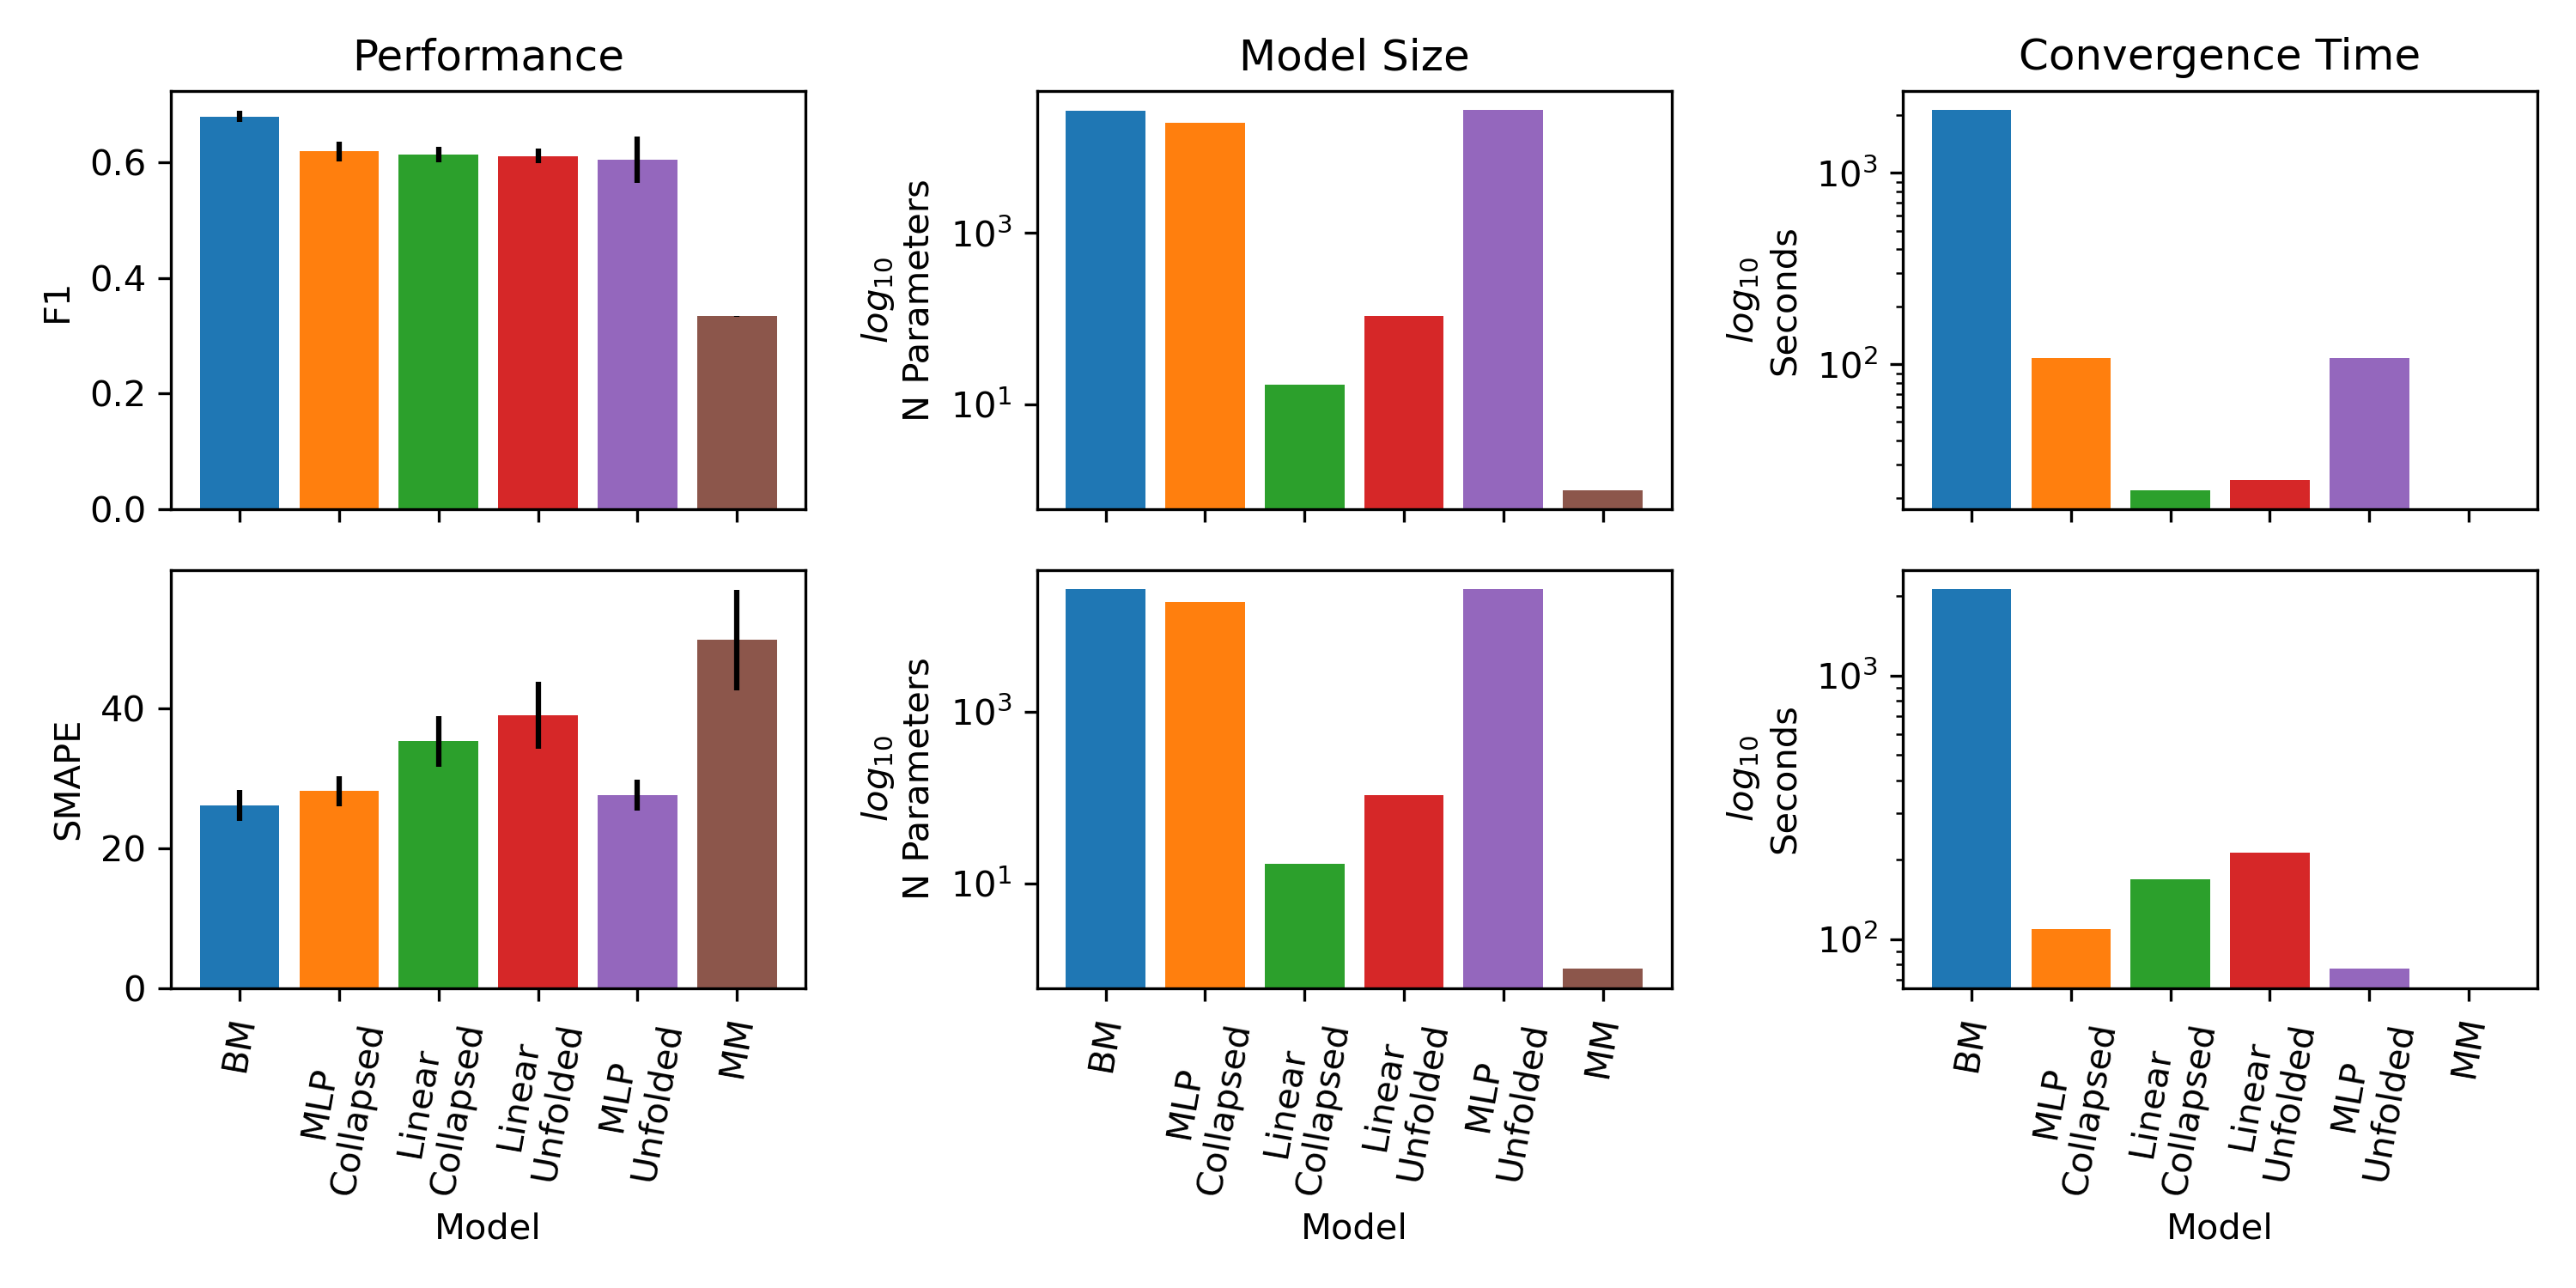
\includegraphics[width=.8\textwidth]{images/chapter_3/global_31.png}
\caption{\textbf{Aggregated comparison of models' performance.}. The BM architecture outperformed all competing ones on both target using however more parameters and computation time. Bar-plots in the first column show the average performance across the 6 game contexts along with estimated standard errors of the mean. The bar-plots on the second and third columns express the number of parameters and the convergence time for each model.}
\label{model_comp_coll_31} 
\end{figure*}
\begin{table}[h]\centering
\caption{\textbf{Performance Baseline Mean Model}}
\label{baseperformance}
\resizebox{0.5\textwidth}{!}{
\begin{tabular}{@{}llrr@{}}
\toprule
\textbf{Game}  &\textbf{Model}                 & \textbf{SMAPE}      & \textbf{F1}       \\ \midrule
\textbf{hmg}   &\multirow{2}{*}{}               & $0.767 \pm 0.001$   & $0.500 \pm 0.003$ \\
\textbf{hms}   &                                & $0.581 \pm 0.001$   & $0.507 \pm 0.003$ \\
\textbf{jc3}   &\multirow{2}{*}{\textbf{MM}}    & $0.632 \pm 0.003$   & $0.499 \pm 0.004$ \\
\textbf{jc4}   &                                & $0.366 \pm 0.002$   & $0.499 \pm 0.001$ \\
\textbf{lis}   &\multirow{2}{*}{\textit{}}      & $0.404 \pm 0.001$   & $0.500 \pm 0.003$ \\
\textbf{lisbf} &                                & $0.244 \pm 0.002$   & $0.500 \pm 0.005$ \\ \bottomrule
\end{tabular}
}
\end{table}
The results from the predictive task carried out using the collapsed dataset, Table \ref{collapsedperformance}, showed how all the 4 models strongly outperformed the MM baseline, Table \ref{baseperformance}, in all games, while also achieving an overall satisfying performance. Moreover we noticed how MLPr and MLPc markedly outperformed EN and LR in both churn probability and survival time prediction across all games.  
\begin{table}[h] \centering
\caption{\textbf{Performance Collapsed Format}}
\label{collapsedperformance}
\resizebox{0.5\textwidth}{!}{
\begin{tabular}{@{}llrlr@{}}
\toprule
\textbf{Game}  &\textbf{Model}                & \textbf{SMAPE}       &\textbf{Model}                & \textbf{F1}       \\ \midrule
\textbf{hmg}   &\multirow{2}{*}{}             & $51.3 \pm 4.3$    &\multirow{2}{*}{}             & $0.591 \pm 0.004$ \\
\textbf{hms}   &                              & $33.1 \pm 2.0$    &                              & $0.624 \pm 0.004$ \\
\textbf{jc3}   &\multirow{2}{*}{\textbf{EN}}  & $42.3 \pm 0.8$    &\multirow{2}{*}{\textbf{LR}}  & $0.601 \pm 0.004$ \\
\textbf{jc4}   &                              & $35.1 \pm 0.6$    &                              & $0.663 \pm 0.002$ \\
\textbf{lis}   &\multirow{2}{*}{}             & $28.7 \pm 0.4$    &\multirow{2}{*}{}             & $0.626 \pm 0.003$ \\
\textbf{lisbf} &                              & $23.9 \pm 0.3$    &                              & $0.591 \pm 0.003$ \\ \midrule

\textbf{hmg}   &\multirow{2}{*}{}             & $30.4 \pm 0.8$    &\multirow{2}{*}{}             & $0.660 \pm 0.006$ \\
\textbf{hms}   &                              & $24.1 \pm 0.7$    &                              & $0.670 \pm 0.006$ \\
\textbf{jc3}   &\multirow{2}{*}{\textbf{MLPr}}& $36.0 \pm 0.3$    &\multirow{2}{*}{\textbf{MLPc}}& $0.654 \pm 0.004$ \\
\textbf{jc4}   &                              & $33.4 \pm 0.2$    &                              & $0.678 \pm 0.004$ \\
\textbf{lis}   &\multirow{2}{*}{\textit{}}    & $25.6 \pm 0.3$    &\multirow{2}{*}{\textit{}}    & $0.664 \pm 0.003$ \\
\textbf{lisbf} &                              & $21.9 \pm 0.2$    &                              & $0.622 \pm 0.003$ \\ \bottomrule
\end{tabular}
}
\end{table}
Looking at the same modelling approaches on the unfolded version of the same dataset we can observed a similar pattern of results, see Table \ref{unfoldedperformance}, regarding baseline and inter-models comparisons. However, it was clear that using unfolded, temporal data lead to only small improvements over the aggregated data. This might be explained by the fact that the chosen modelling approaches are not explicitly designed for taking temporal structure into account, for example they have no explicit mechanics for temporal modelling such as those provided by a LSTM.
\begin{table}[h] \centering
\caption{\textbf{Performance Unfolded Format}}
\label{unfoldedperformance}
\resizebox{0.5\textwidth}{!}{
\begin{tabular}{@{}llrlr@{}}
\toprule
\textbf{Game}  &\textbf{Model}                 & \textbf{SMAPE}  &\textbf{Model}               & \textbf{F1}       \\ \midrule
\textbf{hmg}   &\multirow{2}{*}{}             & $54.5 \pm 2.4$ &\multirow{2}{*}{}             & $0.612 \pm 0.004$ \\
\textbf{hms}   &                              & $55.0 \pm 2.0$ &                              & $0.626 \pm 0.004$ \\
\textbf{jc3}   &\multirow{2}{*}{\textbf{EN}}  & $38.4 \pm 0.3$ &\multirow{2}{*}{\textbf{LR}}  & $0.607 \pm 0.003$ \\
\textbf{jc4}   &                              & $34.9 \pm 0.2$ &                              & $0.660 \pm 0.003$ \\
\textbf{lis}   &\multirow{2}{*}{}             & $30.2 \pm 0.1$ &\multirow{2}{*}{}             & $0.641 \pm 0.004$ \\
\textbf{lisbf} &                              & $23.5 \pm 0.2$ &                              & $0.578 \pm 0.003$ \\ \midrule
\textbf{hmg}   &\multirow{2}{*}{}             & $29.3 \pm 0.4$ &\multirow{2}{*}{}             & $0.683 \pm 0.005$ \\
\textbf{hms}   &                              & $22.6 \pm 0.4$ &                              & $0.682 \pm 0.004$ \\
\textbf{jc3}   &\multirow{2}{*}{\textbf{MLPr}}& $36.0 \pm 0.3$ &\multirow{2}{*}{\textbf{MLPc}}& $0.643 \pm 0.004$ \\
\textbf{jc4}   &                              & $33.1 \pm 0.2$ &                              & $0.681 \pm 0.003$ \\
\textbf{lis}   &\multirow{2}{*}{\textit{}}    & $25.6 \pm 0.2$ &\multirow{2}{*}{\textit{}}    & $0.673 \pm 0.005$ \\
\textbf{lisbf} &                              & $21.8 \pm 0.1$ &                              & $0.627 \pm 0.003$ \\ \bottomrule
\end{tabular}
}
\end{table}
Indeed, when evaluating the performance of the BM, Table \ref{bifurcatingperformance}, on the unfolded data we can see how the model achieves consistent improvements in both churn probability and survival time prediction in all game contexts compared to the previous best model (MLPr and MLPc). From a visual inspection of Figure \ref{perfsurv} 
\begin{figure}[h]
  \centering
  \includegraphics[width=8.5cm]{images/chapter_3/perfromance_survival_31.pdf}
  \caption{\textbf{Performance of the BM on survival task}. The scatter plot shows the relationship between the survival time prediction provided by the BM and the ground truth values. Since the relationship is evaluated on the $log$ of both variables, due to the presence extreme outliers in the ground truth, this acts as mostly as a qualitative complement to the more reliable SMAPE measure.}
  \label{perfsurv}
\end{figure}
we can see the presence of a positive linear relationship between estimated and ground truth survival time (indicative of accordance between the two), with a roughly even distribution of error along the entire range of values. In Table \ref{confusionmatrix} \begin{table}[h] \centering
\caption[\textbf{Performance of the BM on churn task}]{Here the diagonal shows the \% of correct predictions for each label across all games.}
\label{confusionmatrix}
\begin{tabular}{llcc}
\toprule
 & & \multicolumn{2}{c}{\textbf{Prediction}} \\ \cmidrule(lr){3-4}
 & & \parbox[c]{1.5cm}{Churner} & \parbox[c]{1.5cm}{Non-Churner} \\ \midrule
\multirow{2}{*}{\rotatebox{90}{\parbox[c]{1.5cm}{\textbf{Ground  Truth}}}} 
&\multirow{2}{*}{Churner}  & \cellcolor{DarkOliveGreen3!69}   &  \cellcolor{DarkOliveGreen3!31}   \\ 
&&\multirow{-2}{*}{\cellcolor{DarkOliveGreen3!69}0.69}& \multirow{-2}{*}{\cellcolor{DarkOliveGreen3!31}0.31}\\
&\multirow{2}{*}{Non-Churner}  &  \cellcolor{DarkOliveGreen3!33}   &  \cellcolor{DarkOliveGreen3!66}   \\ 
&  &  \multirow{-2}{*}{\cellcolor{DarkOliveGreen3!33} 0.33} & \multirow{-2}{*}{\cellcolor{DarkOliveGreen3!66} 0.66}\\
\bottomrule
\end{tabular}
\end{table} 
we can observe how the model performance is evenly split across the two classes highlighting similar levels of precision and recall. Finally, observing the density plots in Figure \ref{fig:densurv} and \ref{fig:denchurn}
\begin{figure}[h]
  \centering
  \subfloat[Survival Estimations]{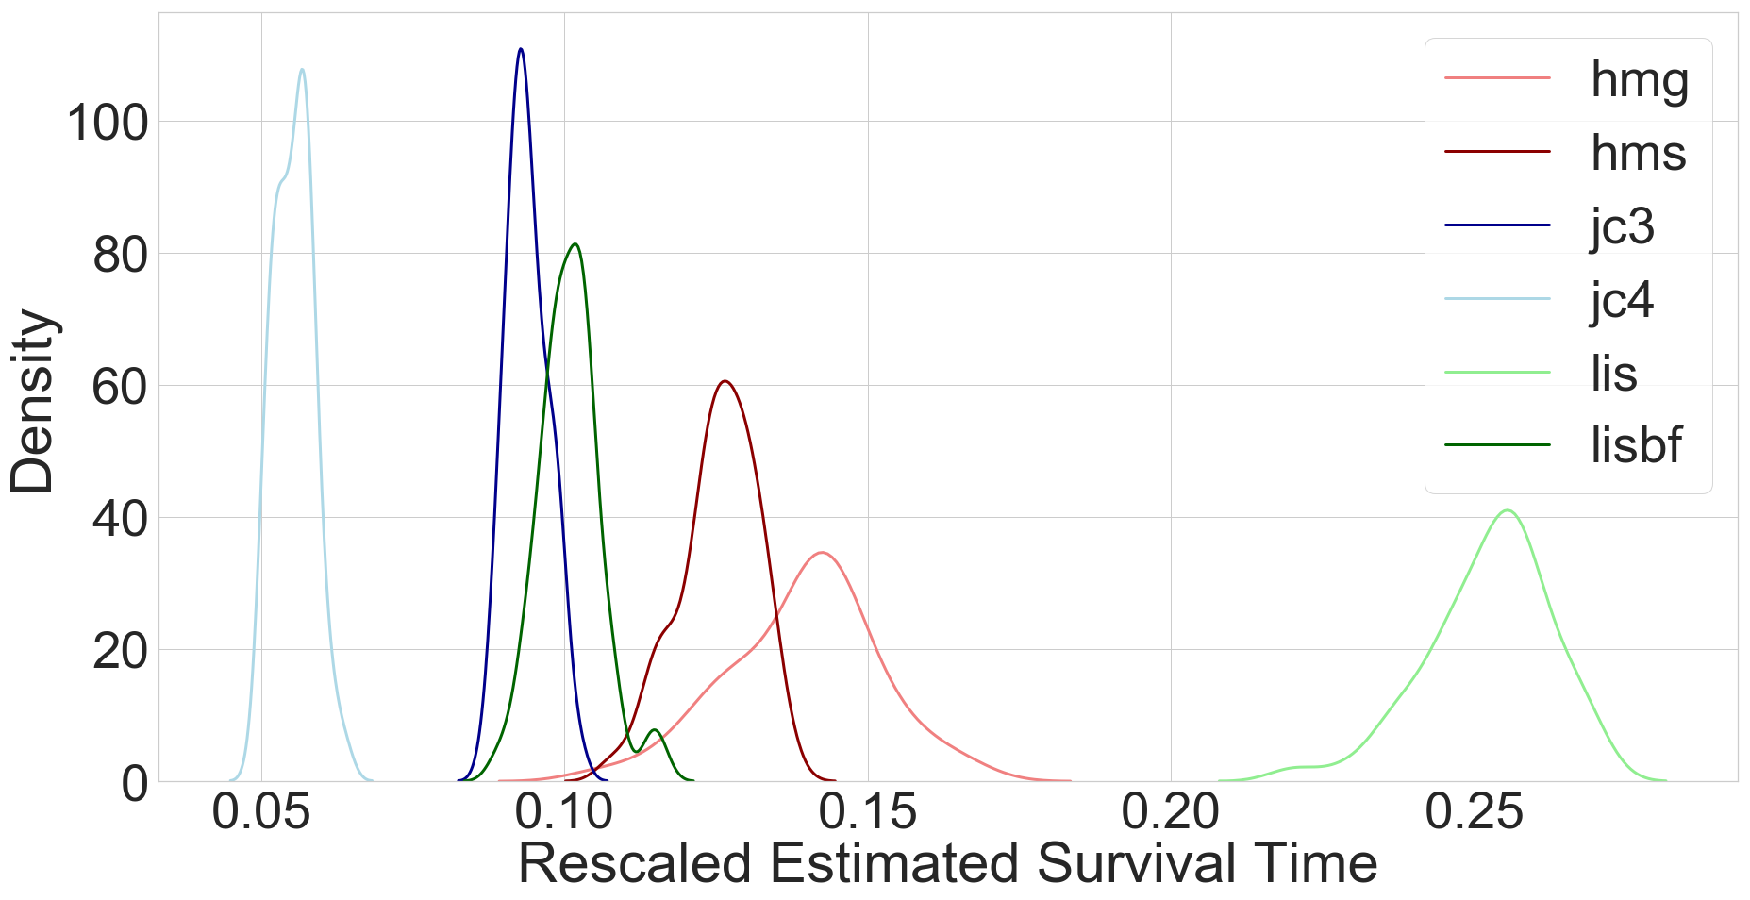
\includegraphics[ width=8.5cm]{images/chapter_3/survival_density_31.pdf}\label{fig:densurv}}
  \hfill
  \subfloat[Churn Probability Estimation]{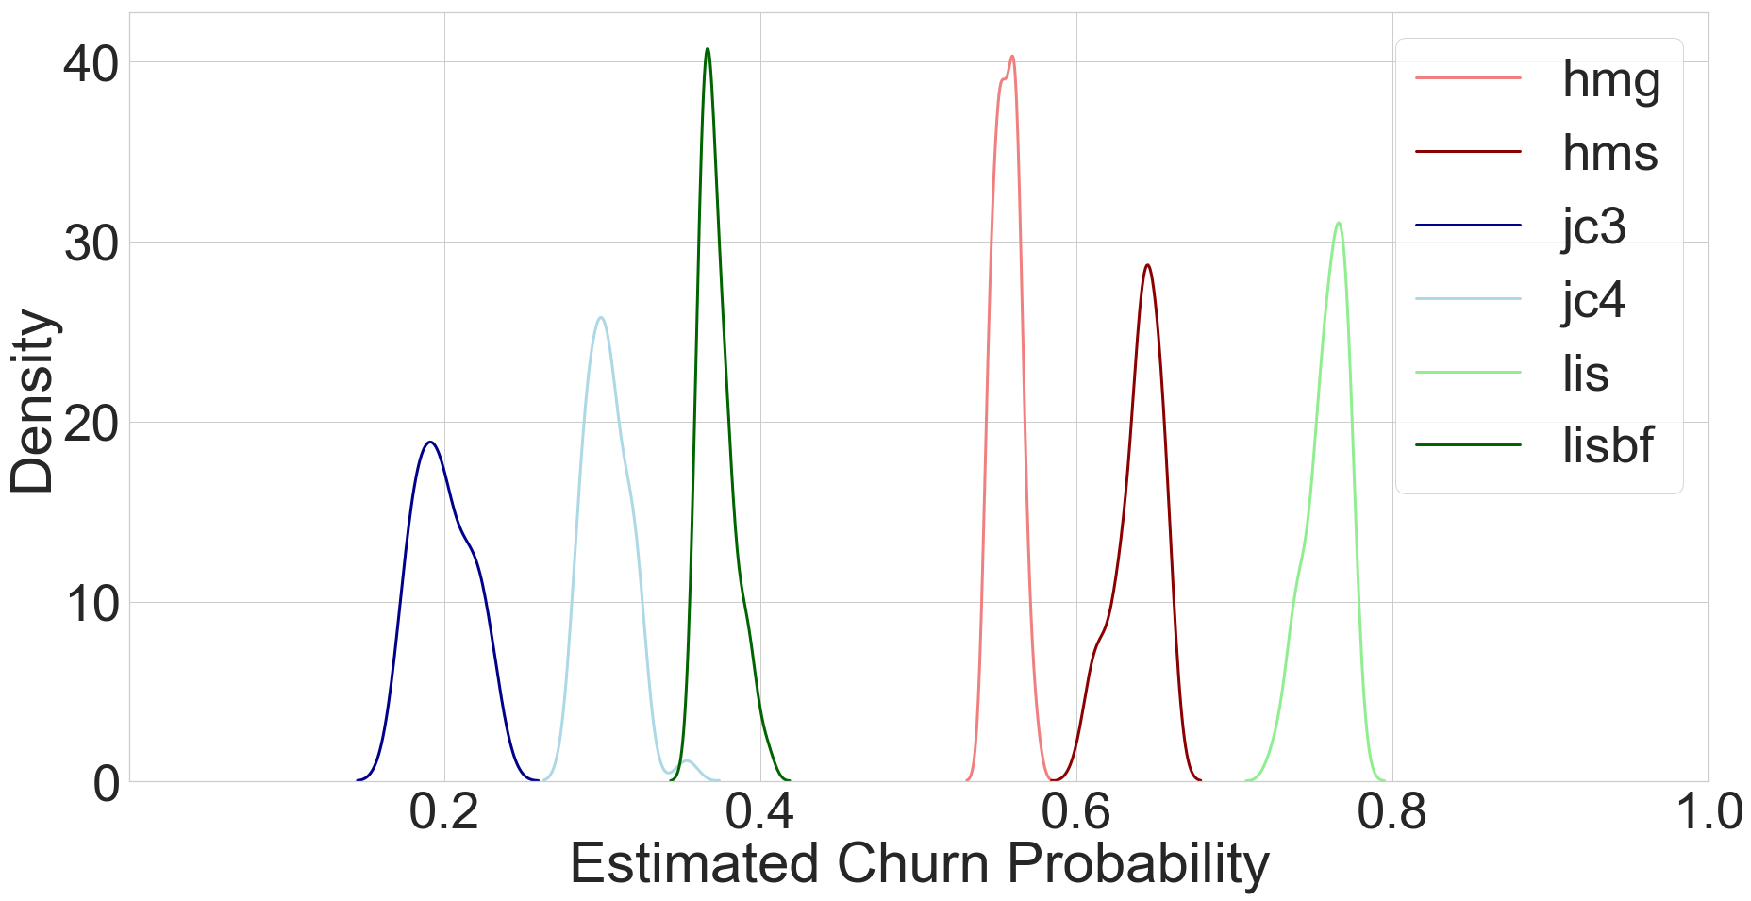
\includegraphics[ width=8.5cm]{images/chapter_3/churn_density_31.pdf}\label{fig:denchurn}}
  \caption{\textbf{Distribution of the BM predictions for six random users, one for each game}. For better comparison the survival estimates are re-scaled game-wise in the range 0 to 1. The highest density point in the distribution represents the most probable predicted value (i.e. the actual prediction),  while the area under the curve instead can be seen as measure of uncertainty (i.e. how confident is the model in its prediction).}
  \label{distestimations}
\end{figure}
we can see how the model was able to encode different levels of uncertainty in the predicted values through different levels of posterior variance.
\begin{table}[h] \centering
\caption{\textbf{Performance Bifurcating Model}}
\label{bifurcatingperformance}
\resizebox{0.5\textwidth}{!}{
\begin{tabular}{@{}llrr@{}}
\toprule
\textbf{Game}  &\textbf{Models}               & \textbf{SMAPE}      & \textbf{F1}       \\ \midrule
\textbf{hmg}   &\multirow{2}{*}{}             & $27.5 \pm 0.1$   & $0.693 \pm 0.002$ \\
\textbf{hms}   &                              & $20.0 \pm 0.1$   & $0.701 \pm 0.003$ \\
\textbf{jc3}   &\multirow{2}{*}{\textbf{BM}}  & $34.4 \pm 0.3$   & $0.671 \pm 0.005$ \\
\textbf{jc4}   &                              & $32.5 \pm 0.2$   & $0.685 \pm 0.002$ \\
\textbf{lis}   &\multirow{2}{*}{}             & $24.6 \pm 0.2$   & $0.688 \pm 0.003$ \\
\textbf{lisbf} &                              & $20.8 \pm 0.1$   & $0.645 \pm 0.003$ \\ \bottomrule
\end{tabular}
}
\end{table}

\subsection{Model Criticism}
The different level of perfromance achieved by the baseline model highlighted how different game context proved to be a more challenging ground (e.g. $jc4$ and $lisbf$) than others with respect to the predictive task. Although we did not perform an exhaustive test for evaluating if disjoint models (i.e. models fitted separately to each game context) would outperform our joint modelling approach, we noticed how each parametric model (which all adopt a joint modelling approach) outperformed the baseline(which adopts a disjoint modelling approach) while maintaining a similar distribution across game contexts. By looking at the perfromance of the various parametric models we saw how  the use of models able to capture non-linear interactions between features provided substantial improvements in predicting measures of future behavioural intensity. We also showed that considering the entire history of individual-games interactions provided a consistent but small edge over metrics representations which are collapsed over time. However, this improvement appeared to be markedly more pronounced and consistent when the predictive task was carried out by non-linear models able to take the dynamical nature of the data into account (e.g. the proposed BM architecture). Finally, by looking more in details at the perfromance of the the BM highlighted how the proposed methodology generalizes well when trying to predict survival time and churn probability as well as successfully incorporating measures of uncertainty in its estimations. In summary, the BM architecture designed following the theoretical principles outlined in chapter \ref{chapter_theory_modelling} showed improved predictive accuracy when compared to alternative with comparable computational expressiveness. That said, it is evident that the architecture doesn't come fully equipped with all the constrains outlined in chapter \ref{chapter_theory_modelling}
and necessary for obtaining a good approximation of the type of construct (i.e. attributed incentive salience) presented in the works of McClure et al. \cite{mcclure2003computational} and Zhang et al. \cite{zhang2009neural}. First of all the BM architecture aims at predicting the accumulated expected ammount of future behaviour at an arbitrary early point in time $t \ll T$ (the OP defined in section \ref{model_design_1}) . This implies that, despite the latent representation generated at time $t$ possesses similar predictive powers to attributed incentive salience, these are not on the same time scale and most importantly are not defined for all the $t \in T$. Second despite churn probability and survival time can be considered good approximations of future behavioural intensity, they surely do not fully capture the complexity of the phenomenon. Moreover, these two metrics can be considered of second order (i.e. they are derived from raw quantifiers of behaviour intensity) and artificially created for serving specific concrete applications in the context of engagement quantification. Since the aim of this thesis is to estimate motivation related latent states (from which, as we said in chapter \ref{chapter_lit_review}, the behavioural manifestation of engagement can be directly derived)) the next iteration in our model building process focused on modifying the BM architecture in order to make its functional form closer to the specifications highlighted in chapter \ref{chapter_theory_modelling}.


\section{Dynamic Prediction of Future Behavioural Intensity}
\label{model_architecture_1}
\lorem

\subsection{Model Design}
Finally to evaluate the effect of recurrency in combination with non-linearity, we designed a hybrid approach (\textit{RNN}) integrating recurrent and feedforward operations in a single ANN. Despite being markedly different, this last architecture shares similarities with the technique proposed by Calhoun et. al. \cite{calhoun2019unsupervised} where latent states were generated dynamically and employed by Generalized Linear Models for producing predictions of observed behaviours. A representation of the computational graphs constituting the parametric models can be seen in Figure \ref{fig: rnn}. It should be noted that E-Net is architecturally equivalent to MLP with the only difference being the replacement of stacked feedforward layers with a single layer with linear activation. As illustrated in Figure \ref{fig: ffnn_rnn} the inputs to each model were sequences of the same behavioural metrics reported in Table \ref{metricsdescription} plus the associated game object while the targets were simply the lead 1 version of the same sequences. We want to highlight how each model was fit to sequences coming from the same game object and that the predictions only pertained the behavioural metrics. Indeed, the aim of each model was to solve
\begin{equation}
    \begin{gathered}
        E(B_{t+1} | \{B_{t}, B_{t-1}, \dots \} , O)
        \label{model_obj}
    \end{gathered}
\end{equation}
jointly for each $O$ present in the data. All the models adopted a multi-task approach (see section \ref{manifold_learning}) and were designed to perform estimation in a sequence-to-sequence fashion: given an input sequence of length $T$ its lead-1 version was predicted. The MLP and RNN models both used a $ReLU$ activation function. The function has shape $ReLU(x) = max(0, x)$ with $x$ being the value computed by a single hidden unit. All the models, except for \textit{Median}, were implemented using Tensorflow's high level API "Keras" \cite{tensorflow2015-whitepaper,chollet2015keras}. The $Median$ model was implemented using the libraries for scientific computing Pandas and Numpy \cite{reback2020pandas,harris2020array}.

\begin{figure}[ht]
\begin{center}
\begin{adjustbox}{width=0.5\textwidth}

   \tikzset{every picture/.style={line width=0.75pt}} %set default line width to 0.75pt        

    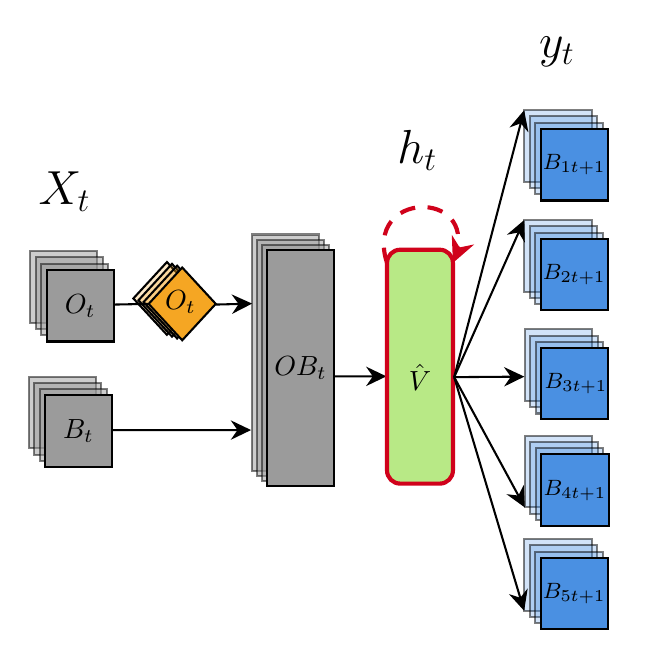
\begin{tikzpicture}[x=0.75pt,y=0.75pt,yscale=-1,xscale=1]
    %uncomment if require: \path (0,354); %set diagram left start at 0, and has height of 354
    
    %Shape: Diamond [id:dp7904557337929367] 
    \draw  [fill={rgb, 255:red, 245; green, 166; blue, 35 }  ,fill opacity=0.25 ] (251.6,119.28) -- (267.77,136.81) -- (251.6,154.33) -- (235.43,136.81) -- cycle ;
    %Shape: Diamond [id:dp44140375398321585] 
    \draw  [fill={rgb, 255:red, 245; green, 166; blue, 35 }  ,fill opacity=0.25 ] (254.05,120.16) -- (270.22,137.68) -- (254.05,155.2) -- (237.89,137.68) -- cycle ;
    %Shape: Diamond [id:dp3808148721846334] 
    \draw  [fill={rgb, 255:red, 245; green, 166; blue, 35 }  ,fill opacity=0.25 ] (256.51,121.04) -- (272.68,138.56) -- (256.51,156.08) -- (240.34,138.56) -- cycle ;
    %Shape: Rectangle [id:dp6212572558437682] 
    \draw  [color={rgb, 255:red, 0; green, 0; blue, 0 }  ,draw opacity=0.5 ][fill={rgb, 255:red, 155; green, 155; blue, 155 }  ,fill opacity=0.5 ] (292.41,106.01) -- (324.92,106.01) -- (324.92,219.74) -- (292.41,219.74) -- cycle ;
    %Shape: Rectangle [id:dp04308865519441296] 
    \draw  [color={rgb, 255:red, 0; green, 0; blue, 0 }  ,draw opacity=0.5 ][fill={rgb, 255:red, 155; green, 155; blue, 155 }  ,fill opacity=0.5 ] (294.86,108.47) -- (327.38,108.47) -- (327.38,222.2) -- (294.86,222.2) -- cycle ;
    %Shape: Rectangle [id:dp692301238884502] 
    \draw  [color={rgb, 255:red, 0; green, 0; blue, 0 }  ,draw opacity=0.5 ][fill={rgb, 255:red, 155; green, 155; blue, 155 }  ,fill opacity=0.5 ] (297.32,110.93) -- (329.84,110.93) -- (329.84,224.66) -- (297.32,224.66) -- cycle ;
    %Shape: Diamond [id:dp3746200743423901] 
    \draw  [fill={rgb, 255:red, 245; green, 166; blue, 35 }  ,fill opacity=1 ] (258.97,121.91) -- (275.13,139.43) -- (258.97,156.96) -- (242.8,139.43) -- cycle ;
    %Straight Lines [id:da9537882301539488] 
    \draw    (274.94,139.77) -- (289.65,139.38) ;
    \draw [shift={(292.65,139.3)}, rotate = 178.49] [fill={rgb, 255:red, 0; green, 0; blue, 0 }  ][line width=0.08]  [draw opacity=0] (9.82,-4.72) -- (0,0) -- (9.82,4.72) -- (6.52,0) -- cycle    ;
    %Straight Lines [id:da45479882207763933] 
    \draw [fill={rgb, 255:red, 155; green, 155; blue, 155 }  ,fill opacity=1 ]   (203.09,200.3) -- (289.13,200.22) ;
    \draw [shift={(292.13,200.22)}, rotate = 179.95] [fill={rgb, 255:red, 0; green, 0; blue, 0 }  ][line width=0.08]  [draw opacity=0] (9.82,-4.72) -- (0,0) -- (9.82,4.72) -- (6.52,0) -- cycle    ;
    %Straight Lines [id:da9952506139878592] 
    \draw [fill={rgb, 255:red, 155; green, 155; blue, 155 }  ,fill opacity=1 ]   (324.42,174.36) -- (354.33,174.35) ;
    \draw [shift={(357.33,174.35)}, rotate = 179.97] [fill={rgb, 255:red, 0; green, 0; blue, 0 }  ][line width=0.08]  [draw opacity=0] (9.82,-4.72) -- (0,0) -- (9.82,4.72) -- (6.52,0) -- cycle    ;
    %Shape: Rectangle [id:dp5105796971723443] 
    \draw  [color={rgb, 255:red, 0; green, 0; blue, 0 }  ,draw opacity=0.5 ][fill={rgb, 255:red, 155; green, 155; blue, 155 }  ,fill opacity=0.5 ] (185.01,174.53) -- (217.26,174.53) -- (217.26,209.05) -- (185.01,209.05) -- cycle ;
    %Shape: Rectangle [id:dp2595806858227925] 
    \draw  [color={rgb, 255:red, 0; green, 0; blue, 0 }  ,draw opacity=0.5 ][fill={rgb, 255:red, 155; green, 155; blue, 155 }  ,fill opacity=0.5 ] (187.63,177.51) -- (219.88,177.51) -- (219.88,212.03) -- (187.63,212.03) -- cycle ;
    %Shape: Rectangle [id:dp8277252726471348] 
    \draw  [color={rgb, 255:red, 0; green, 0; blue, 0 }  ,draw opacity=0.5 ][fill={rgb, 255:red, 155; green, 155; blue, 155 }  ,fill opacity=0.5 ] (190.27,180.56) -- (222.53,180.56) -- (222.53,215.08) -- (190.27,215.08) -- cycle ;
    %Shape: Rectangle [id:dp4311381435790056] 
    \draw  [fill={rgb, 255:red, 155; green, 155; blue, 155 }  ,fill opacity=1 ] (192.86,183.5) -- (225.11,183.5) -- (225.11,218.02) -- (192.86,218.02) -- cycle ;
    %Shape: Rectangle [id:dp5047118561624738] 
    \draw  [fill={rgb, 255:red, 155; green, 155; blue, 155 }  ,fill opacity=1 ] (299.77,113.39) -- (332.29,113.39) -- (332.29,227.12) -- (299.77,227.12) -- cycle ;
    %Shape: Rectangle [id:dp21573647855268596] 
    \draw  [color={rgb, 255:red, 0; green, 0; blue, 0 }  ,draw opacity=0.5 ][fill={rgb, 255:red, 155; green, 155; blue, 155 }  ,fill opacity=0.5 ] (185.83,114.08) -- (218.08,114.08) -- (218.08,148.6) -- (185.83,148.6) -- cycle ;
    %Shape: Rectangle [id:dp8439578107486148] 
    \draw  [color={rgb, 255:red, 0; green, 0; blue, 0 }  ,draw opacity=0.5 ][fill={rgb, 255:red, 155; green, 155; blue, 155 }  ,fill opacity=0.5 ] (188.45,117.06) -- (220.7,117.06) -- (220.7,151.58) -- (188.45,151.58) -- cycle ;
    %Shape: Rectangle [id:dp3660318943838672] 
    \draw  [color={rgb, 255:red, 0; green, 0; blue, 0 }  ,draw opacity=0.5 ][fill={rgb, 255:red, 155; green, 155; blue, 155 }  ,fill opacity=0.5 ] (191.09,120.11) -- (223.35,120.11) -- (223.35,154.63) -- (191.09,154.63) -- cycle ;
    %Shape: Rectangle [id:dp7778058544321894] 
    \draw  [fill={rgb, 255:red, 155; green, 155; blue, 155 }  ,fill opacity=1 ] (193.68,123.05) -- (225.93,123.05) -- (225.93,157.57) -- (193.68,157.57) -- cycle ;
    %Straight Lines [id:da7015539931476137] 
    \draw    (225.82,139.77) -- (242.8,139.43) ;
    %Rounded Rect [id:dp4473399888202214] 
    \draw  [color={rgb, 255:red, 208; green, 2; blue, 27 }  ,draw opacity=1 ][fill={rgb, 255:red, 184; green, 233; blue, 134 }  ,fill opacity=1 ][line width=1.5]  (357.64,119.69) .. controls (357.64,116.18) and (360.48,113.34) .. (363.99,113.34) -- (383.05,113.34) .. controls (386.56,113.34) and (389.4,116.18) .. (389.4,119.69) -- (389.4,219.68) .. controls (389.4,223.19) and (386.56,226.03) .. (383.05,226.03) -- (363.99,226.03) .. controls (360.48,226.03) and (357.64,223.19) .. (357.64,219.68) -- cycle ;
    %Curve Lines [id:da30430836514862303] 
    \draw [color={rgb, 255:red, 208; green, 2; blue, 27 }  ,draw opacity=1 ][line width=1.5]  [dash pattern={on 5.63pt off 4.5pt}]  (357.64,119.69) .. controls (346.28,85.07) and (400.82,83.85) .. (390.76,116.05) ;
    \draw [shift={(389.4,119.69)}, rotate = 293.32] [fill={rgb, 255:red, 208; green, 2; blue, 27 }  ,fill opacity=1 ][line width=0.08]  [draw opacity=0] (12.23,-5.88) -- (0,0) -- (12.23,5.88) -- (8.12,0) -- cycle    ;
    %Shape: Rectangle [id:dp9161667828288995] 
    \draw  [color={rgb, 255:red, 0; green, 0; blue, 0 }  ,draw opacity=0.5 ][fill={rgb, 255:red, 74; green, 144; blue, 226 }  ,fill opacity=0.25 ] (423.7,99.06) -- (456.2,99.06) -- (456.2,133.57) -- (423.7,133.57) -- cycle ;
    %Shape: Rectangle [id:dp20889912329934768] 
    \draw  [color={rgb, 255:red, 0; green, 0; blue, 0 }  ,draw opacity=0.5 ][fill={rgb, 255:red, 74; green, 144; blue, 226 }  ,fill opacity=0.25 ] (426.34,102.04) -- (458.84,102.04) -- (458.84,136.54) -- (426.34,136.54) -- cycle ;
    %Shape: Rectangle [id:dp2816776467625347] 
    \draw  [color={rgb, 255:red, 0; green, 0; blue, 0 }  ,draw opacity=0.5 ][fill={rgb, 255:red, 74; green, 144; blue, 226 }  ,fill opacity=0.25 ] (429,105.09) -- (461.51,105.09) -- (461.51,139.6) -- (429,139.6) -- cycle ;
    %Shape: Rectangle [id:dp42330781005921503] 
    \draw  [fill={rgb, 255:red, 74; green, 144; blue, 226 }  ,fill opacity=1 ] (431.61,108.03) -- (464.11,108.03) -- (464.11,142.53) -- (431.61,142.53) -- cycle ;
    %Shape: Rectangle [id:dp687693866282439] 
    \draw  [color={rgb, 255:red, 0; green, 0; blue, 0 }  ,draw opacity=0.5 ][fill={rgb, 255:red, 74; green, 144; blue, 226 }  ,fill opacity=0.25 ] (424.03,151.72) -- (456.53,151.72) -- (456.53,186.23) -- (424.03,186.23) -- cycle ;
    %Shape: Rectangle [id:dp48312027278133507] 
    \draw  [color={rgb, 255:red, 0; green, 0; blue, 0 }  ,draw opacity=0.5 ][fill={rgb, 255:red, 74; green, 144; blue, 226 }  ,fill opacity=0.25 ] (426.67,154.7) -- (459.17,154.7) -- (459.17,189.21) -- (426.67,189.21) -- cycle ;
    %Shape: Rectangle [id:dp5685283982245644] 
    \draw  [color={rgb, 255:red, 0; green, 0; blue, 0 }  ,draw opacity=0.5 ][fill={rgb, 255:red, 74; green, 144; blue, 226 }  ,fill opacity=0.25 ] (429.33,157.76) -- (461.84,157.76) -- (461.84,192.26) -- (429.33,192.26) -- cycle ;
    %Shape: Rectangle [id:dp3612684141121718] 
    \draw  [fill={rgb, 255:red, 74; green, 144; blue, 226 }  ,fill opacity=1 ] (431.95,160.69) -- (464.17,160.69) -- (464.17,194.89) -- (431.95,194.89) -- cycle ;
    %Shape: Rectangle [id:dp17418879327554693] 
    \draw  [color={rgb, 255:red, 0; green, 0; blue, 0 }  ,draw opacity=0.5 ][fill={rgb, 255:red, 74; green, 144; blue, 226 }  ,fill opacity=0.25 ] (423.7,252.78) -- (456.2,252.78) -- (456.2,287.29) -- (423.7,287.29) -- cycle ;
    %Shape: Rectangle [id:dp6752714184560265] 
    \draw  [color={rgb, 255:red, 0; green, 0; blue, 0 }  ,draw opacity=0.5 ][fill={rgb, 255:red, 74; green, 144; blue, 226 }  ,fill opacity=0.25 ] (426.34,255.76) -- (458.84,255.76) -- (458.84,290.26) -- (426.34,290.26) -- cycle ;
    %Shape: Rectangle [id:dp9983191940012098] 
    \draw  [color={rgb, 255:red, 0; green, 0; blue, 0 }  ,draw opacity=0.5 ][fill={rgb, 255:red, 74; green, 144; blue, 226 }  ,fill opacity=0.25 ] (429,258.81) -- (461.51,258.81) -- (461.51,293.32) -- (429,293.32) -- cycle ;
    %Shape: Rectangle [id:dp11003700320217247] 
    \draw  [fill={rgb, 255:red, 74; green, 144; blue, 226 }  ,fill opacity=1 ] (431.61,261.75) -- (464.11,261.75) -- (464.11,296.25) -- (431.61,296.25) -- cycle ;
    %Shape: Rectangle [id:dp7367493878137299] 
    \draw  [color={rgb, 255:red, 0; green, 0; blue, 0 }  ,draw opacity=0.5 ][fill={rgb, 255:red, 74; green, 144; blue, 226 }  ,fill opacity=0.25 ] (424.03,202.99) -- (456.53,202.99) -- (456.53,237.5) -- (424.03,237.5) -- cycle ;
    %Shape: Rectangle [id:dp8983348276713422] 
    \draw  [color={rgb, 255:red, 0; green, 0; blue, 0 }  ,draw opacity=0.5 ][fill={rgb, 255:red, 74; green, 144; blue, 226 }  ,fill opacity=0.25 ] (426.67,205.97) -- (459.17,205.97) -- (459.17,240.47) -- (426.67,240.47) -- cycle ;
    %Shape: Rectangle [id:dp09933660328753013] 
    \draw  [color={rgb, 255:red, 0; green, 0; blue, 0 }  ,draw opacity=0.5 ][fill={rgb, 255:red, 74; green, 144; blue, 226 }  ,fill opacity=0.25 ] (429.33,209.02) -- (461.84,209.02) -- (461.84,243.53) -- (429.33,243.53) -- cycle ;
    %Shape: Rectangle [id:dp9943795167198757] 
    \draw  [fill={rgb, 255:red, 74; green, 144; blue, 226 }  ,fill opacity=1 ] (431.94,211.96) -- (464.44,211.96) -- (464.44,246.46) -- (431.94,246.46) -- cycle ;
    %Shape: Rectangle [id:dp058820430549127] 
    \draw  [color={rgb, 255:red, 0; green, 0; blue, 0 }  ,draw opacity=0.5 ][fill={rgb, 255:red, 74; green, 144; blue, 226 }  ,fill opacity=0.25 ] (423.7,46.14) -- (456.2,46.14) -- (456.2,80.65) -- (423.7,80.65) -- cycle ;
    %Shape: Rectangle [id:dp9593581977954196] 
    \draw  [color={rgb, 255:red, 0; green, 0; blue, 0 }  ,draw opacity=0.5 ][fill={rgb, 255:red, 74; green, 144; blue, 226 }  ,fill opacity=0.25 ] (426.34,49.12) -- (458.84,49.12) -- (458.84,83.63) -- (426.34,83.63) -- cycle ;
    %Shape: Rectangle [id:dp4362593009406618] 
    \draw  [color={rgb, 255:red, 0; green, 0; blue, 0 }  ,draw opacity=0.5 ][fill={rgb, 255:red, 74; green, 144; blue, 226 }  ,fill opacity=0.25 ] (429,52.17) -- (461.51,52.17) -- (461.51,86.68) -- (429,86.68) -- cycle ;
    %Shape: Rectangle [id:dp7619519997532663] 
    \draw  [fill={rgb, 255:red, 74; green, 144; blue, 226 }  ,fill opacity=1 ] (431.61,55.11) -- (464.11,55.11) -- (464.11,89.62) -- (431.61,89.62) -- cycle ;
    %Straight Lines [id:da545267197618029] 
    \draw    (390,174.73) -- (422.94,49.05) ;
    \draw [shift={(423.7,46.14)}, rotate = 104.68] [fill={rgb, 255:red, 0; green, 0; blue, 0 }  ][line width=0.08]  [draw opacity=0] (9.82,-4.72) -- (0,0) -- (9.82,4.72) -- (6.52,0) -- cycle    ;
    %Straight Lines [id:da9271821433537066] 
    \draw    (390,174.73) -- (422.48,101.8) ;
    \draw [shift={(423.7,99.06)}, rotate = 114] [fill={rgb, 255:red, 0; green, 0; blue, 0 }  ][line width=0.08]  [draw opacity=0] (9.82,-4.72) -- (0,0) -- (9.82,4.72) -- (6.52,0) -- cycle    ;
    %Straight Lines [id:da6232303168074279] 
    \draw    (390,174.73) -- (420.8,174.5) ;
    \draw [shift={(423.8,174.48)}, rotate = 179.57] [fill={rgb, 255:red, 0; green, 0; blue, 0 }  ][line width=0.08]  [draw opacity=0] (9.82,-4.72) -- (0,0) -- (9.82,4.72) -- (6.52,0) -- cycle    ;
    %Straight Lines [id:da1424758683168187] 
    \draw    (390,174.73) -- (422.6,234.86) ;
    \draw [shift={(424.03,237.5)}, rotate = 241.54] [fill={rgb, 255:red, 0; green, 0; blue, 0 }  ][line width=0.08]  [draw opacity=0] (9.82,-4.72) -- (0,0) -- (9.82,4.72) -- (6.52,0) -- cycle    ;
    %Straight Lines [id:da40105840572004403] 
    \draw    (390,174.73) -- (422.84,284.41) ;
    \draw [shift={(423.7,287.29)}, rotate = 253.33] [fill={rgb, 255:red, 0; green, 0; blue, 0 }  ][line width=0.08]  [draw opacity=0] (9.82,-4.72) -- (0,0) -- (9.82,4.72) -- (6.52,0) -- cycle    ;
    
    % Text Node
    \draw (208.99,200.76) node  [font=\normalsize]  {$B_{t}$};
    % Text Node
    \draw (373.52,174.8) node  [font=\normalsize]  {$\hat{V}$};
    % Text Node
    \draw (258.15,138.56) node  [font=\normalsize]  {$O_{t}$};
    % Text Node
    \draw (202.34,85.25) node  [font=\LARGE]  {$X_{t}$};
    % Text Node
    \draw (316.03,170.25) node  [font=\normalsize]  {$OB_{t}$};
    % Text Node
    \draw (209.81,140.31) node  [font=\normalsize]  {$O_{t}$};
    % Text Node
    \draw (372.34,65.6) node  [font=\LARGE]  {$h_{t}$};
    % Text Node
    \draw (447.86,125.28) node  [font=\footnotesize]  {$B_{2t+1}$};
    % Text Node
    \draw (448.74,177.94) node  [font=\footnotesize]  {$B_{3t+1}$};
    % Text Node
    \draw (448.19,229.21) node  [font=\footnotesize]  {$B_{4t+1}$};
    % Text Node
    \draw (447.86,279) node  [font=\footnotesize]  {$B_{5t+1}$};
    % Text Node
    \draw (439.54,18) node  [font=\LARGE]  {$y_{t}$};
    % Text Node
    \draw (447.86,72.36) node  [font=\footnotesize]  {$B_{1t+1}$};
    
    
    \end{tikzpicture}


\end{adjustbox}
\end{center}
\caption[\textbf{The recurrent architecture}]{Blue, orange and green shapes represent respectively feedforward, embedding and LSTM operations. Gray shapes indicate operations with no learnable parameters, such as tensor instantiation and concatenation. Stacked, transparent colouring indicates tensors with a sequential structure. Straight and curved arrows refer to the presence of feed-forward or recurrent information flow. The red highlight shows the portion of the model we hypothesize is inferring an approximation of attributed incentive salience.}
\label{fig: rnn_2}
\end{figure}

\subsection{Data}
To validate our approach and hypotheses we needed to acquire records of interactions between individuals and potentially rewarding objects in naturalistic contexts. As mentioned in section \ref{videogame_telemetries}, video games are particularly suited for this purpose given their learning-dependent reinforcing properties and the large amount of longitudinal data streams that they can generate. We used gameplay data from  six video games published by our partner company, \textit{Square Enix Ltd.}. The games were \emph{Hitman Go} (hmg), \emph{Hitman Sniper} (hms), \emph{Just Cause 3} (jc3), \emph{Just Cause 4} (jc4), \emph{Life is Strange} (lis), and \emph{Life is Strange: Before the Storm} (lisbf). Due to the diversity in their in-game mechanics, each of these games was considered as an "object" with different reinforcing properties (see section \ref{videogame_telemetries}). This allowed us to mimic a situation where a single model had access to data coming from a heterogeneous set of potentially rewarding entities (similarly to what we described in section \ref{motivation}). The resulting dataset contained entries from 3,209,336 individuals, evenly distributed across the six games, and randomly sampled from all users who played the games between their respective release date and January 2020. All data were obtained and processed in compliance with the European Union's General Data Protection Regulation \cite{EUdataregulations2018}. In order to represent state transition dynamics (i.e. sequences of interactions between $I$ and $O$) for each individual, we retrieved a set of six different types of behavioural telemetry over variable-length sequences of game sessions. A game session was defined from the moment an individual started the game software until it was closed. We retrieved all sessions produced by an individual from the moment the data they generated first appeared in the game's servers. Since our modelling approach requires to predict, in a supervised manner, the intensity of future playing behaviour given the history of previous interactions, we only considered users with two or more observed game sessions. The reason for this is two fold: sequences of length one do not entail any temporal structure and do not allow to generate a supervised target.
\begin{table}[H] \centering
\caption{\textbf{Description of Selected Telemetries}}
\label{metricsdescription_2}
  \begin{tabularx}{\textwidth}{@{}lX@{}}
    \toprule
    \textbf{Metric}      & \textbf{Description}          \\ \midrule
    {Absence}    & Temporal distance between sessions (hours)  \\
    {Session Time}     & Overall session duration (minutes)       \\ 
    {Active Time}      & Percentage of Session Time actively playing  \\ 
    {Session Activity}    & Count of user initiated gameplay-related actions. E.g.\\ 
                & "Attack an enemy" is considered a valid\\ 
                & action while "Being attacked by an enemy" is not.\\
    {N°Sessions}    & Number of played sessions.\\ 
    {Object}    &  Game object identifier.  \\
    \bottomrule
  \end{tabularx}
\end{table}
The telemetry (see Table \ref{metricsdescription}) were selected to be generalizable and comparable with metrics employed in other behavioural studies of incentive salience attribution \cite{berridge1998role,mcclure2003computational,zhang2009neural}. We note that the high dispersion values (Inter Quartile Range  or IQR), reported for some of the telemetry are due to the extreme skewness in the distribution of the data. This is caused both by the nature of the phenomenon they describe (e.g. Absence is a classic case of time-to-event measure) and by their typical behaviour in the context of videogames \cite{bauckhage2012players}. The final dataset was composed of 6 columns and 28,155,199 rows. A table of descriptive statistics can be found in \ref{game_description}.

\begin{table*}[h]
\centering
\caption{Descriptive Statistics of Considered Metrics and Games}
\label{game_description}
  \resizebox{0.8\textwidth}{!}{
  \begin{tabular}{cccccccc}
  \toprule
  \multirow{2}{*}{\textbf{Game}} &
   \multirow{2}{*}{\textbf{\begin{tabular}[c]{@{}c@{}}Sample \\ Size\end{tabular}}} &
   \textbf{\begin{tabular}[c]{@{}c@{}}Number \\ of \\ Sessions\end{tabular}} &
   \textbf{\begin{tabular}[c]{@{}c@{}}Absence \\ (minutes)\end{tabular}} &
   \textbf{\begin{tabular}[c]{@{}c@{}}Session \\ Time\\ (minutes)\end{tabular}} &
   \textbf{\begin{tabular}[c]{@{}c@{}}Active \\ Time\\ (\% Session Time)\end{tabular}} &
   \textbf{\begin{tabular}[c]{@{}c@{}}Session \\ Activity\end{tabular}} &
   \multirow{2}{*}{\textbf{\begin{tabular}[c]{@{}c@{}}Game \\ Description\end{tabular}}} \\ \midrule
   &
    &
   \multicolumn{5}{c}{\textbf{\begin{tabular}[c]{@{}c@{}}(Median $\pm$ IQR)\end{tabular}}} &
    \\ \midrule
  \textbf{hmg} &
   501,649 &
   \begin{tabular}[c]{@{}c@{}}3 $\pm$ 3\end{tabular} &
   \begin{tabular}[c]{@{}c@{}}84$\pm$ 2,169\end{tabular} &
   \begin{tabular}[c]{@{}c@{}}22 $\pm$ 22 \end{tabular} &
   \begin{tabular}[c]{@{}c@{}}64 $\pm$  42 \end{tabular} &
   \begin{tabular}[c]{@{}c@{}}25 $\pm$  31\end{tabular} &
   \begin{tabular}[c]{@{}c@{}}Mobile\\ Strategy\end{tabular} \\
  \textbf{hms} &
   504,504 &
   \begin{tabular}[c]{@{}c@{}}8 $\pm$ 9\end{tabular} &
   \begin{tabular}[c]{@{}c@{}}24 $\pm$ 198\end{tabular} &
   \begin{tabular}[c]{@{}c@{}}28 $\pm$ 8\end{tabular} &
   \begin{tabular}[c]{@{}c@{}}42 $\pm$ 35\end{tabular} &
   \begin{tabular}[c]{@{}c@{}}6 $\pm$ 8 \end{tabular} &
   \begin{tabular}[c]{@{}c@{}}Mobile\\ Shooting Gallery\end{tabular} \\
  \textbf{jc3} &
   540,000 &
   \begin{tabular}[c]{@{}c@{}}7 $\pm$ 8\end{tabular} &
   \begin{tabular}[c]{@{}c@{}}64 $\pm$ 488\end{tabular} &
   \begin{tabular}[c]{@{}c@{}}162 $\pm$ 23\end{tabular} &
   \begin{tabular}[c]{@{}c@{}}60 $\pm$ 55\end{tabular} &
   \begin{tabular}[c]{@{}c@{}}19 $\pm$ 23\end{tabular} &
   \begin{tabular}[c]{@{}c@{}}Console\\ Action Open World\end{tabular} \\
  \textbf{jc4} &
   571,501 &
   \begin{tabular}[c]{@{}c@{}}5 $\pm$ 6 \end{tabular} &
   \begin{tabular}[c]{@{}c@{}}64 $\pm$ 406\end{tabular} &
   \begin{tabular}[c]{@{}c@{}}133 $\pm$ 64\end{tabular} &
   \begin{tabular}[c]{@{}c@{}}43 $\pm$ 46\end{tabular} &
   \begin{tabular}[c]{@{}c@{}}46 $\pm$ 64\end{tabular} &
   \begin{tabular}[c]{@{}c@{}}Console\\ Action Open World\end{tabular} \\
  \textbf{lis} &
   533,364 &
   \begin{tabular}[c]{@{}c@{}}4 $\pm$ 4\end{tabular} &
   \begin{tabular}[c]{@{}c@{}}143  $\pm$ 3,004\end{tabular} &
   \begin{tabular}[c]{@{}c@{}}96 $\pm$ 50\end{tabular} &
   \begin{tabular}[c]{@{}c@{}}48 $\pm$ 44\end{tabular} &
   \begin{tabular}[c]{@{}c@{}}40 $\pm$ 50\end{tabular} &
   \begin{tabular}[c]{@{}c@{}}Console\\ Graphic Adventure\end{tabular} \\
  \textbf{lisbf} &
   517,782 &
   \begin{tabular}[c]{@{}c@{}}4 $\pm$ 5\end{tabular} &
   \begin{tabular}[c]{@{}c@{}}71 $\pm$ 1,162\end{tabular} &
   \begin{tabular}[c]{@{}c@{}}102 $\pm$ 32\end{tabular} &
   \begin{tabular}[c]{@{}c@{}}79 $\pm$ 20\end{tabular} &
   \begin{tabular}[c]{@{}c@{}}23 $\pm$ 32\end{tabular} &
   \begin{tabular}[c]{@{}c@{}}Console\\ Graphic Adventure\end{tabular} \\ \bottomrule
  \end{tabular}
  }
\end{table*}

\subsection{Model Comparison}
When querying the data from the game servers, we excluded from the random sampling procedure individuals having at least one of the considered behavioural metrics over the game population's \nth{99} percentile. This allowed us to eliminate potentially faulty data which are often present when dealing with telemetry. At this point data were re-arranged in a format suitable for time series modelling (i.e. arrays of shape $(batch\times T \times B)$ with $T$ being the number of available game sessions and $B$ the number of considered behavioural metrics) and randomly split into a tuning (i.e. 10 \%) and validation set (i.e. 90 \%). For the sake of clarity we report an example of how the data from a game session are generated and how they are parsed by the models.\\
\\
\textit{
"A user decides, 36 hours after the release of game X, to enter the game world for the first time. This is when a session starts and actual playing behaviour can be observed. During this session they engage in various activities leading to 20 non-unique and user-initiated actions (e.g. being attacked by a non-playable character is not counted as a valid action). After roughly 60 minutes spent playing, the user exits the game world and the session ends. Of this session, 80\% of time has been spent actively playing, the remaining 20\% has seen the game on pause or the user away from the console (i.e. idle time). After 48 hours the user logs into the game world again and a new session starts"}\\
\\
What we described here would correspond to a single time step $t_{1}$ in the sequence $T$ of total interactions (i.e. sessions) between the user and the specific game context X. The models will parse this session as a vector of length 4 with values 36, 20, 60, 80 and 20 along with another vector of length 1 containing the numerical index for the game. When all the sessions are observed the models will receive as inputs sequences of length $T$ of the same vectors. 

\paragraph{\textbf{Performance Analysis}} 
\label{perf_analysis}
The first step in our performance analysis aimed to control for the contribution of hyper-parameters in the performance of the parametric models (especially for MLP and RNN). The choice of factors such as the number of layers and hidden units can influence the number of free parameters and expressive power of an ANN. Manually picking their optimal value is often a challenging combinatorial problem that can lead to unexpected outcomes if left to the subjective choice of the experimenter. Therefore, to find the best hyperparameters we adopted a more impartial and efficient approach relying on algorithmic search. This was done using the Keras Tuner implementation \cite{omalley2019kerastuner} of the Hyperband algorithm \cite{li2017hyperband}. Hyperband is an optimized version of random search that achieves faster convergence through adaptive resources allocation and early termination of training. It can lead to better or equivalent results to other optimization algorithms but in a fraction of the time \cite{li2017hyperband}. When initializing the tuning step we allowed each model to grow as much as the others (except for E-Net, which,  due to the fact that it is a linear model, is naturally constrained to a fixed number of parameters) so that any observed difference in number of parameters was related to characteristics of the model architecture. The tuning step was conducted running one full iteration of Hyperband with a budget of 40 epochs \footnote{See  \cite{li2017hyperband,hyperwebs} for a detailed description of the Hyperband technique.} on the tuning set. To trigger early stopping for a specific configuration of hyperparameters, we monitored the decrease in loss over a 20\% random sample of the tuning set (i.e. the validation tuning set) and we terminated training when the loss reduced by less than $\delta = 1\mathrm{e}{-4}$ for 10 consecutive epochs. Once the best set of hyperparameters was found we proceeded to fit all the models specified in section \ref{models} on the training set using a 10-fold Cross Validation Strategy. This  divided the validation set in 10 equally sized folds and iteratively used 9 of them for training and 1 for testing. The continuous inputs in the training data were min-max scaled according to the formula
\begin{equation}
  \begin{gathered} 
  \label{min_max}
        MinMax(x) =\frac{x - \min(x)} {\max(x) - \min(x)} 
  \end{gathered}
\end{equation}
where $x$ is the input vector to be scaled, while the categorical input (i.e. game object) was encoded ordinally. In order to take into account the contributions of time, game and target, the performance of each model was given by computing the Symmetric Mean Percentage Error (SMAPE) \cite{zhu2017deep} for each combination of the aforementioned dimensions (e.g. SMAPE of Session Time at $t1$ for the game object hmg). Each model was trained for a maximum of 200 epochs and interrupted using the same early stopping strategy mentioned above (i.e. absence of $\delta$ reduction in loss on a 20\% hold-out for 10 consecutive epochs). To maintain the ability to fit each model on temporal series of varying length, we adopted a data generator approach \footnote{See \cite{chollet2015keras,tensorflow2015-whitepaper} for implementation details.} feeding data to the models in random batches of 256 time series with constant length within a batch. The models were trained with stochastic gradient descent using the Adaptive Moment Estimation (Adam) \cite{kingma2014adam} algorithm to find the set of parameters minimizing the SMAPE between the targets and the predictions generated by the model. The choice of SMAPE was dictated by the fact that the targets were expressed on largely different scales (i.e. coming from different games and expressed on different units of measure see Table \ref{metricsdescription}) and therefore required a loss function measuring relative distance from the target. To evaluate the overall performance, we first summed the SMAPE relative to each target in a single global performance indicator: this is the loss function that each model attempts to minimize during training. W then divided the total by 5 (i.e. the total number of targets) in order to express the metric in its original scale (i.e. 0 to 100). This was then regressed using a Linear Mixed-effects Model (LMM) with fold number, game object and time as random effects and model type as fixed effect (treatment coded with RNN as reference). Subsequently, for a more thorough investigation of model performance we conducted the same regression analysis separately on each target. Both regression analyses were followed by post-hoc comparisons (i.e. t-tests with Bonferroni correction) for testing the following pairwise hypotheses on the estimated coefficients: Lag 1 $<$ Median $<$ ENet $<$ MLP. All statistical analyses were conducted using the python library statsmodels \cite{seabold2010statsmodels}. 

\subsection{Models} 
\label{models}
When defining the models used for evaluating our hypotheses, we first established two reasonable single-parameter baselines. The first is a \textit{Lag 1} model producing predictions according to the following rule:
\begin{equation}
   \begin{gathered}  
     B_{t+1} = B_{t}
     \label{lag_1}
  \end{gathered}
\end{equation}
here $t$ represent a single game session in a sequence of $T$ observed interactions while $B$ are the behavioural metrics described in section \ref{data}. The second is a \textit{Median} model computing the expectancy of each of the 4 targets according to the formula:
\begin{equation}
  \begin{gathered}  
    \overline{B_{t+1}} = \frac
      {\sum_{i=1}^{t+1} wB_{i}}
      {\sum_{i=1}^{t+1} w }\\
    B_{t+1} = median(\overline{B_{t+1}}) 
    \label{median}
  \end{gathered}
\end{equation}
here $\overline{B_{t+1}}$ is an exponentially weighted average of all the $B_t$ up to $t+1$ observed when fitting the model. This is computed separately for every individual in the dataset and the median value of each of the 4 targets is used a a constant prediction. These apparently naive models provide a surprisingly robust prediction baseline for time series that are not white noise \cite{hyndman2018forecasting} other than having a nice interpretation in terms of behavioural momentum \cite{nevin2000behavioral}: in conditions of high experienced reward the behaviour of an individual tends to be consistent over time (i.e. resistant to change). An ElasticNet (\textit{E-Net}) \cite{zou2005regularization}, a form of additive model combining both $l1$ and $l2$ regularization, was used to evaluate the performance of simple linear functions. To test the effect of non linearity, a Multilayer Perceptron (\textit{MLP}), the most common type of deep feedforward ANN, was used. 

\subsection{Results}
At the level of global performance the RNN model markedly outperformed all competing approaches as clearly shown in Figure \ref{model_comp_coll}. This can be also seen in the results of the regression (see Table \ref{collapsed_target_lmm}) and  \textit{post hoc} analysis (see Table \ref{collapsed_target_lmm_post_hoc}). From the \textit{post hoc} analysis we can also observe how all the pairwise hypotheses presented in paragraph \ref{perf_analysis} are confirmed. Here model performance is given by the sum of all the losses produced by the five targets and therefore provides a general indicator of model fit where lower values indicate a better performance overall.

\begin{figure}[h]
\centering
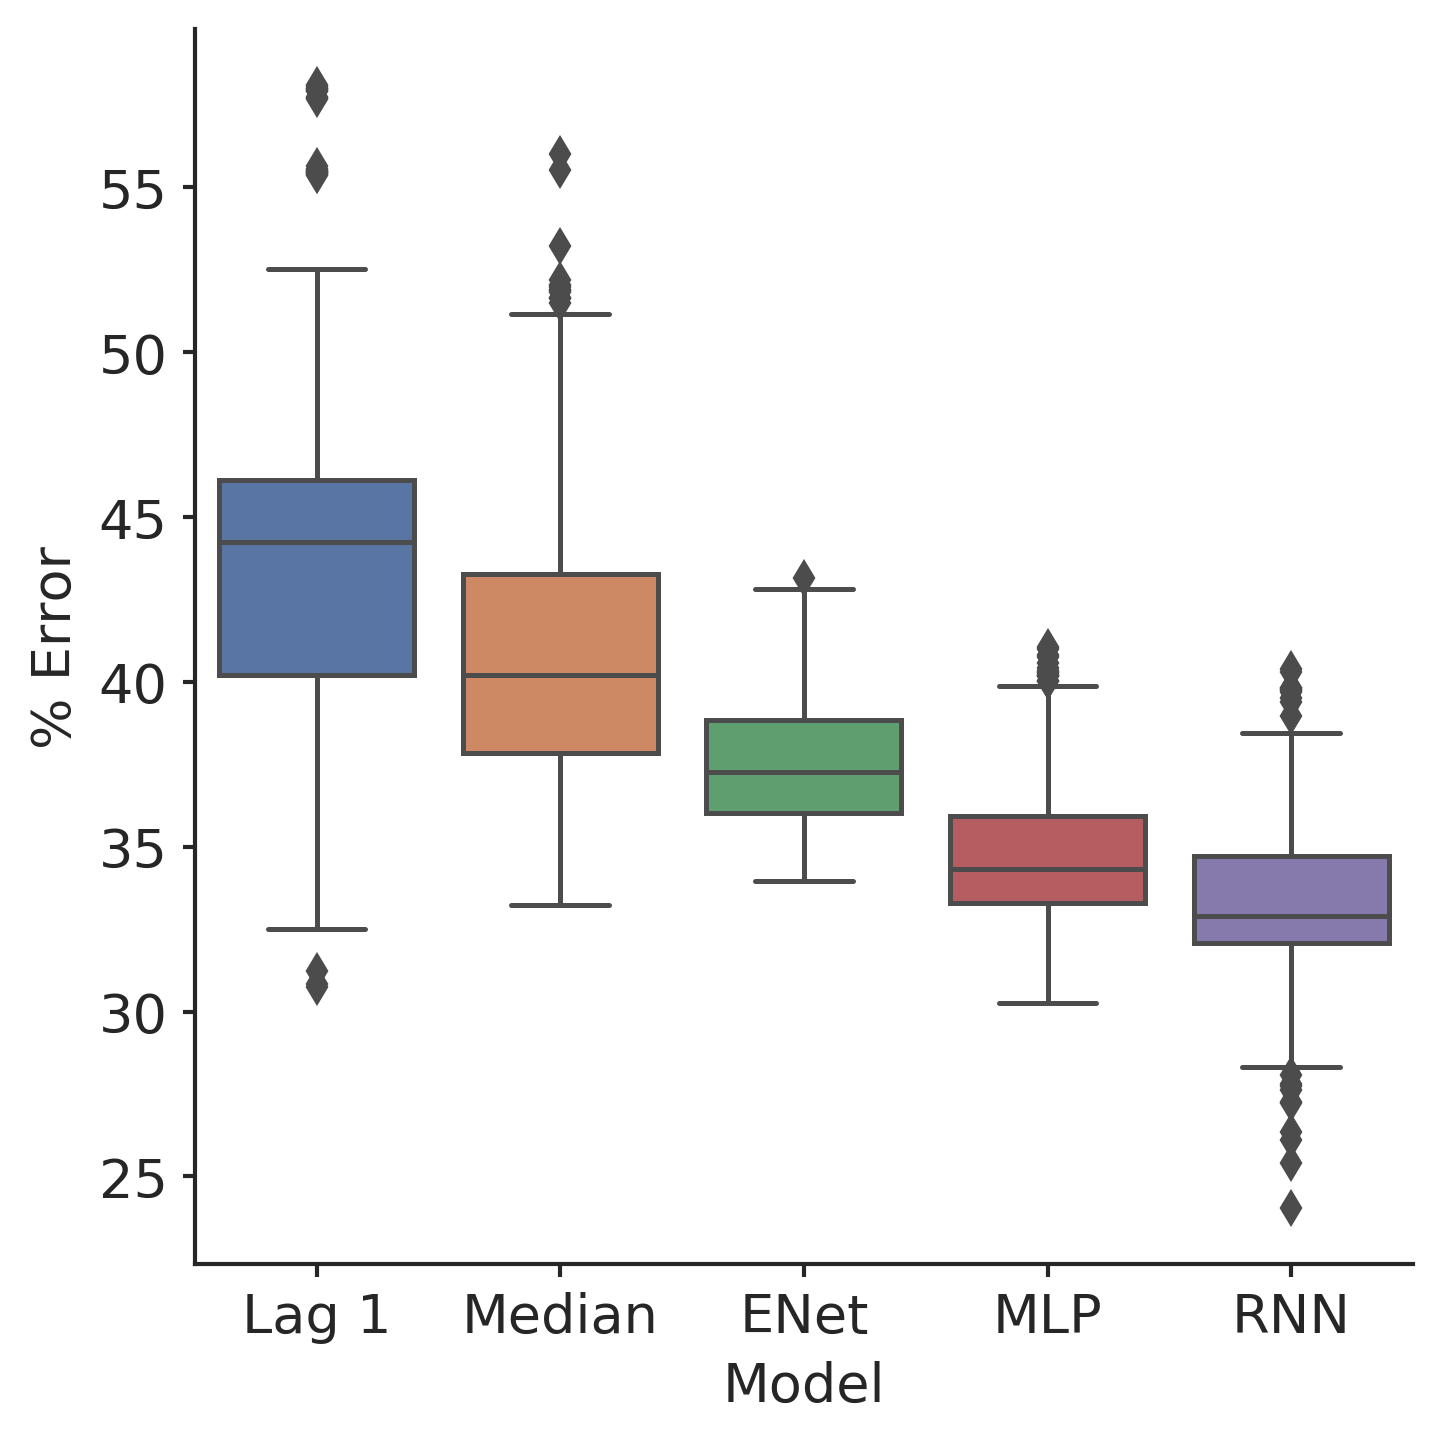
\includegraphics[width=.5\columnwidth]{images/chapter_3/performance_collapsed_32.png}
\caption{\textbf{Aggregated comparison of model performance.} Overall, our approach (RNN) outperforms all the competing approaches. Box-plots show the 10-fold cross-validation performance expressed as the total percentage of error (i.e. SMAPE) of each model over the five targets.}
\label{model_comp_coll} 
\end{figure}

\begin{table}[h]
\centering
\caption{Results of LMM on Collapsed Targets (Sum)}
\label{collapsed_target_lmm}
\resizebox{0.5\textwidth}{!}{
\begin{tabular}{ccccc}
\hline
\textbf{Model}           & \textbf{$\beta$} & \textbf{Z} & \textbf{p} & \textbf{95\% C.I.} \\ \hline
\multicolumn{5}{c}{\textbf{Collapsed Targets (Sum)}}                                                 \\ \hline
\textbf{Intercept (RNN)} & 33.129                & 41.799     & \textless .01   & 31.575 - 34.682      \\
\textbf{Lag 1}           & 10.010                 & 80.023     & \textless .01   & 9.765 - 10.255        \\
\textbf{Median}          & 7.482                 & 59.813     & \textless .01   & 7.237 - 7.727        \\
\textbf{ENet}            & 4.189                 & 33.491     & \textless .01   & 3.944 - 4.435        \\
\textbf{MLP}             & 1.411                 & 11.280     & \textless .01   & 1.166 - 1.656        \\ \hline
\end{tabular}
}
\end{table}
\begin{table}[h]
\centering
\caption{LMM Post-Hoc on Collapsed Targets (Sum)}
\label{collapsed_target_lmm_post_hoc}
\begin{tabular}{ccccc}
\hline
\textbf{Contrast}           & \textbf{$\beta_1$ - $\beta_2$} & \textbf{Z} & \textbf{p} & \textbf{95\% C.I.} \\ \hline
\multicolumn{5}{c}{\textbf{Collapsed Targets (Sum)}}                                                 \\ \hline
\textbf{Lag 1 - Median} & 2.528                & 20.210     & \textless .01   & 2.283 - 2.773      \\
\textbf{Median - ENet}          & 3.292                 & 26.322     & \textless .01   & 3.048 - 3.538        \\
\textbf{ENet - MLP}          & 2.778                 & 22.211     & \textless .01   & 2.533 - 3.024        \\ \hline
\end{tabular}
\end{table}

The superiority of the RNN model can still be observed when comparing the models on each target separately. However, the size of the effect varies depending on the target (see Table \ref{exploded_target_lmm}). The same trend is also present in the \textit{post hoc} analysis (see Table \ref{exploded_target_lmm_post_hoc}) where we observe only a partial confirmation of the pairwise hypotheses. The ENet model is outperformed by the Median baseline for three targets, namely Future Active Time, Session Time and Session Activity. All the coefficients in the regression analyses and the differences in the \textit{post hoc} analyses are non-standardized and can be interpreted as absolute changes in percentage error (i.e. SMAPE). In order to make these values more easily interpretable, we can use the information Table \ref{game_description}. For example, knowing that the median Session Time for the jc3 object is 162 minutes we can derive that when the RNN model achieves a SMAPE of 30\% in predicting Future Session Time, this equates on average to an absolute error of $1.62 \times 30 \sim 48$ minutes. All the p-values in the \textit{post hoc} analyses are Bonferroni corrected for multiple comparisons. The results of the statistical analyses suggest positive additive effects of non-linearity and recurrency on model performance both at the level of global and target-specific performance. This effect is more pronounced for certain targets (e.g. Future Session Time, Future N° Sessions) than for others (e.g. Future Absence, Future Active Time). Moreover, looking at Figure \ref{model_comp_non_coll} it appears that RNN improved on MLP (i.e. the second best model) using roughly half the parameters and per-epoch computation time. This could indicate that recurrency both improves model fit and allows for more efficient use of the available parameters.

\begin{table}[h]
\centering
\caption{Results of LMM on Non-Collapsed Targets}
\label{exploded_target_lmm}
\begin{tabular}{ccccc}
\hline
\textbf{Model}  & \textbf{$\beta$} & \textbf{Z} & \textbf{p} & \textbf{95\% C.I.}                  \\ \hline
\multicolumn{5}{c}{\textbf{Future Absence}}                                                                         \\ \hline
\textbf{Intercept (RNN)} & 54.46                & 144.316     & \textless .01   & 53.72 - 55.20                     \\
\textbf{Lag 1}           & 7.40                & 40.509     & \textless .01   & 7.04 - 7.76                     \\
\textbf{Median}          & 9.47                & 51.814     & \textless .01   & 9.11 - 9.83                     \\
\textbf{ENet}            & 1.71                & 9.353     & \textless .01   & 1.35 - 2.06                     \\
\textbf{MLP}             & .53                & 2.915     & \textless .01   & .175 - .891                       \\ \hline
\multicolumn{5}{c}{\textbf{Future Active Time}}                                                                     \\ \hline
\textbf{Intercept (RNN)} & 23.36                & 20.019      & \textless .01  & 21.78 - 24.93                     \\
\textbf{Lag 1}           & 7.32               & 119.028    & \textless .01  & 7.2 - 7.44                     \\
\textbf{Median}          & .77                & 12.515     & \textless .01  & .649 - .891                     \\
\textbf{ENet}            & 2.55                & 41.551     & \textless .01  & 2.43 - 2.67                     \\
\textbf{MLP}             & .41                & 6.739      & \textless .01  & .294 - .535                     \\ \hline
\multicolumn{5}{c}{\textbf{Future Session Time}}                                                                     \\ \hline
\textbf{Intercept (RNN)} & 30.02                & 63.663     & \textless .01  & 29.1 - 30.95                     \\
\textbf{Lag 1}            & 5.62                & 49.158     & \textless .01  & 5.39 - 5.83                     \\
\textbf{Median}          & 4.45                & 38.957     & \textless .01  & 4.23 - 4.67                     \\
\textbf{ENet}            & 4.81                & 42.098     & \textless .01  & 4.59 - 5.03                     \\
\textbf{MLP}             & 1.08                & 9.529      & \textless .01  & .86 - 1.31                     \\ \hline
\multicolumn{5}{c}{\textbf{Future Session Activity}}                                                                 \\ \hline
\textbf{Intercept (RNN)} & 31.04                & 70.241     & \textless .01  & \multicolumn{1}{l}{30.17 - 31.9} \\
\textbf{Lag 1}            & 6.52                & 61.025     & \textless .01  & \multicolumn{1}{l}{6.31 - 6.73} \\
\textbf{Median}          & 4.37                & 40.879     & \textless .01  & \multicolumn{1}{l}{4.16 - 4.58} \\
\textbf{ENet}            & 4.42                & 41.319     & \textless .01  & \multicolumn{1}{l}{4.21 - 4.63} \\
\textbf{MLP}             & 1.36                & 12.762     & \textless .01  & \multicolumn{1}{l}{1.15 - 1.57} \\ \hline
\multicolumn{5}{c}{\textbf{Future N° Sessions}}                                                                      \\ \hline
\textbf{Intercept (RNN)} & 26.77                & 7.445     & \textless .01  & 19.72 - 33.81                     \\
\textbf{Lag 1}            & 23.17                & 44.430     & \textless .01  & 22.15 - 24.19                     \\
\textbf{Median}          &  18.34              & 35.166     & \textless .01  & 17.31 - 19.36                     \\
\textbf{ENet}            & 7.44                & 14.277     & \textless .01  & 6.42 - 8.46                     \\
\textbf{MLP}             & 3.65                & 7.005      & \textless .01  & 2.63 - 4.67                       \\ \hline
\end{tabular}
\end{table}
\begin{table}[h]
\centering
\caption{LMM Post-Hoc on Non-Collapsed Targets}
\label{exploded_target_lmm_post_hoc}
\begin{tabular}{ccccc}
\hline
\textbf{Contrast}  & \textbf{$\beta_1$-$\beta_2$} & \textbf{Z} & \textbf{p} & \textbf{95\% C.I.}                  \\ \hline
\multicolumn{5}{c}{\textbf{Future Absence}}                                                                         \\ \hline
\textbf{Lag 1 - Median} & -2.06                & -11.305     & \textless .01   & -2.42 - -1.70                     \\
\textbf{Median - ENet}           & 7.76                & 42.461     & \textless .01   & 7.40 - 8.12                     \\
\textbf{ENet - MLP}          & 1.17                & 6.438     & \textless .01   & .81 - 1.535                    \\ \hline
\multicolumn{5}{c}{\textbf{Future Active Time}}                                                                     \\ \hline
\textbf{Lag 1 - Median} & 6.55                & 106.513      & \textless .01  & 6.433 - 6.67                     \\
\textbf{Median - ENet}           & -1.78                & -29.037    & \textless .01  & -1.9 - -1.66                     \\
\textbf{ENet - MLP}          & 2.14                & 34.812     & \textless .01  & 2.02 - 2.26                     \\\hline
\multicolumn{5}{c}{\textbf{Future Session Time}}                                                                     \\ \hline
\textbf{Lag 1 - Median} & 1.16                & 10.201     & \textless .01  & .94 - 1.39                     \\
\textbf{Median - ENet}            & -.35                & -3.141     & \textless .01  & -.58 - -.13                     \\
\textbf{ENet - MLP}          & 3.72                & 32.579     & \textless .01  & 3.5 - 3.95                     \\ \hline
\multicolumn{5}{c}{\textbf{Future Session Activity}}                                                                 \\ \hline
\textbf{Lag 1 - Median} & 2.15                & 20.146     & \textless .01  & \multicolumn{1}{l}{1.94 - 2.36} \\
\textbf{Median - ENet}            & -.04                & -.441     &  1.  & \multicolumn{1}{l}{-.257 - .163} \\
\textbf{ENet - MLP}          & 3.05                & 28.558     & \textless .01  & \multicolumn{1}{l}{2.84 - 3.26} \\ \hline
\multicolumn{5}{c}{\textbf{Future N° Sessions}}                                                                      \\ \hline
\textbf{Lag 1 - Median} & 4.83                & 9.264     & \textless .01  & 3.8 - 5.85                     \\
\textbf{Median - ENet}            & 10.89                & 20.889     & \textless .01  & 9.87 - 11.91                     \\
\textbf{ENet - MLP}          & 3.79                & 7.272     & \textless .01  & 2.77 - 4.81                     \\\hline
\end{tabular}
\end{table}

\begin{figure*}[h]
\centering
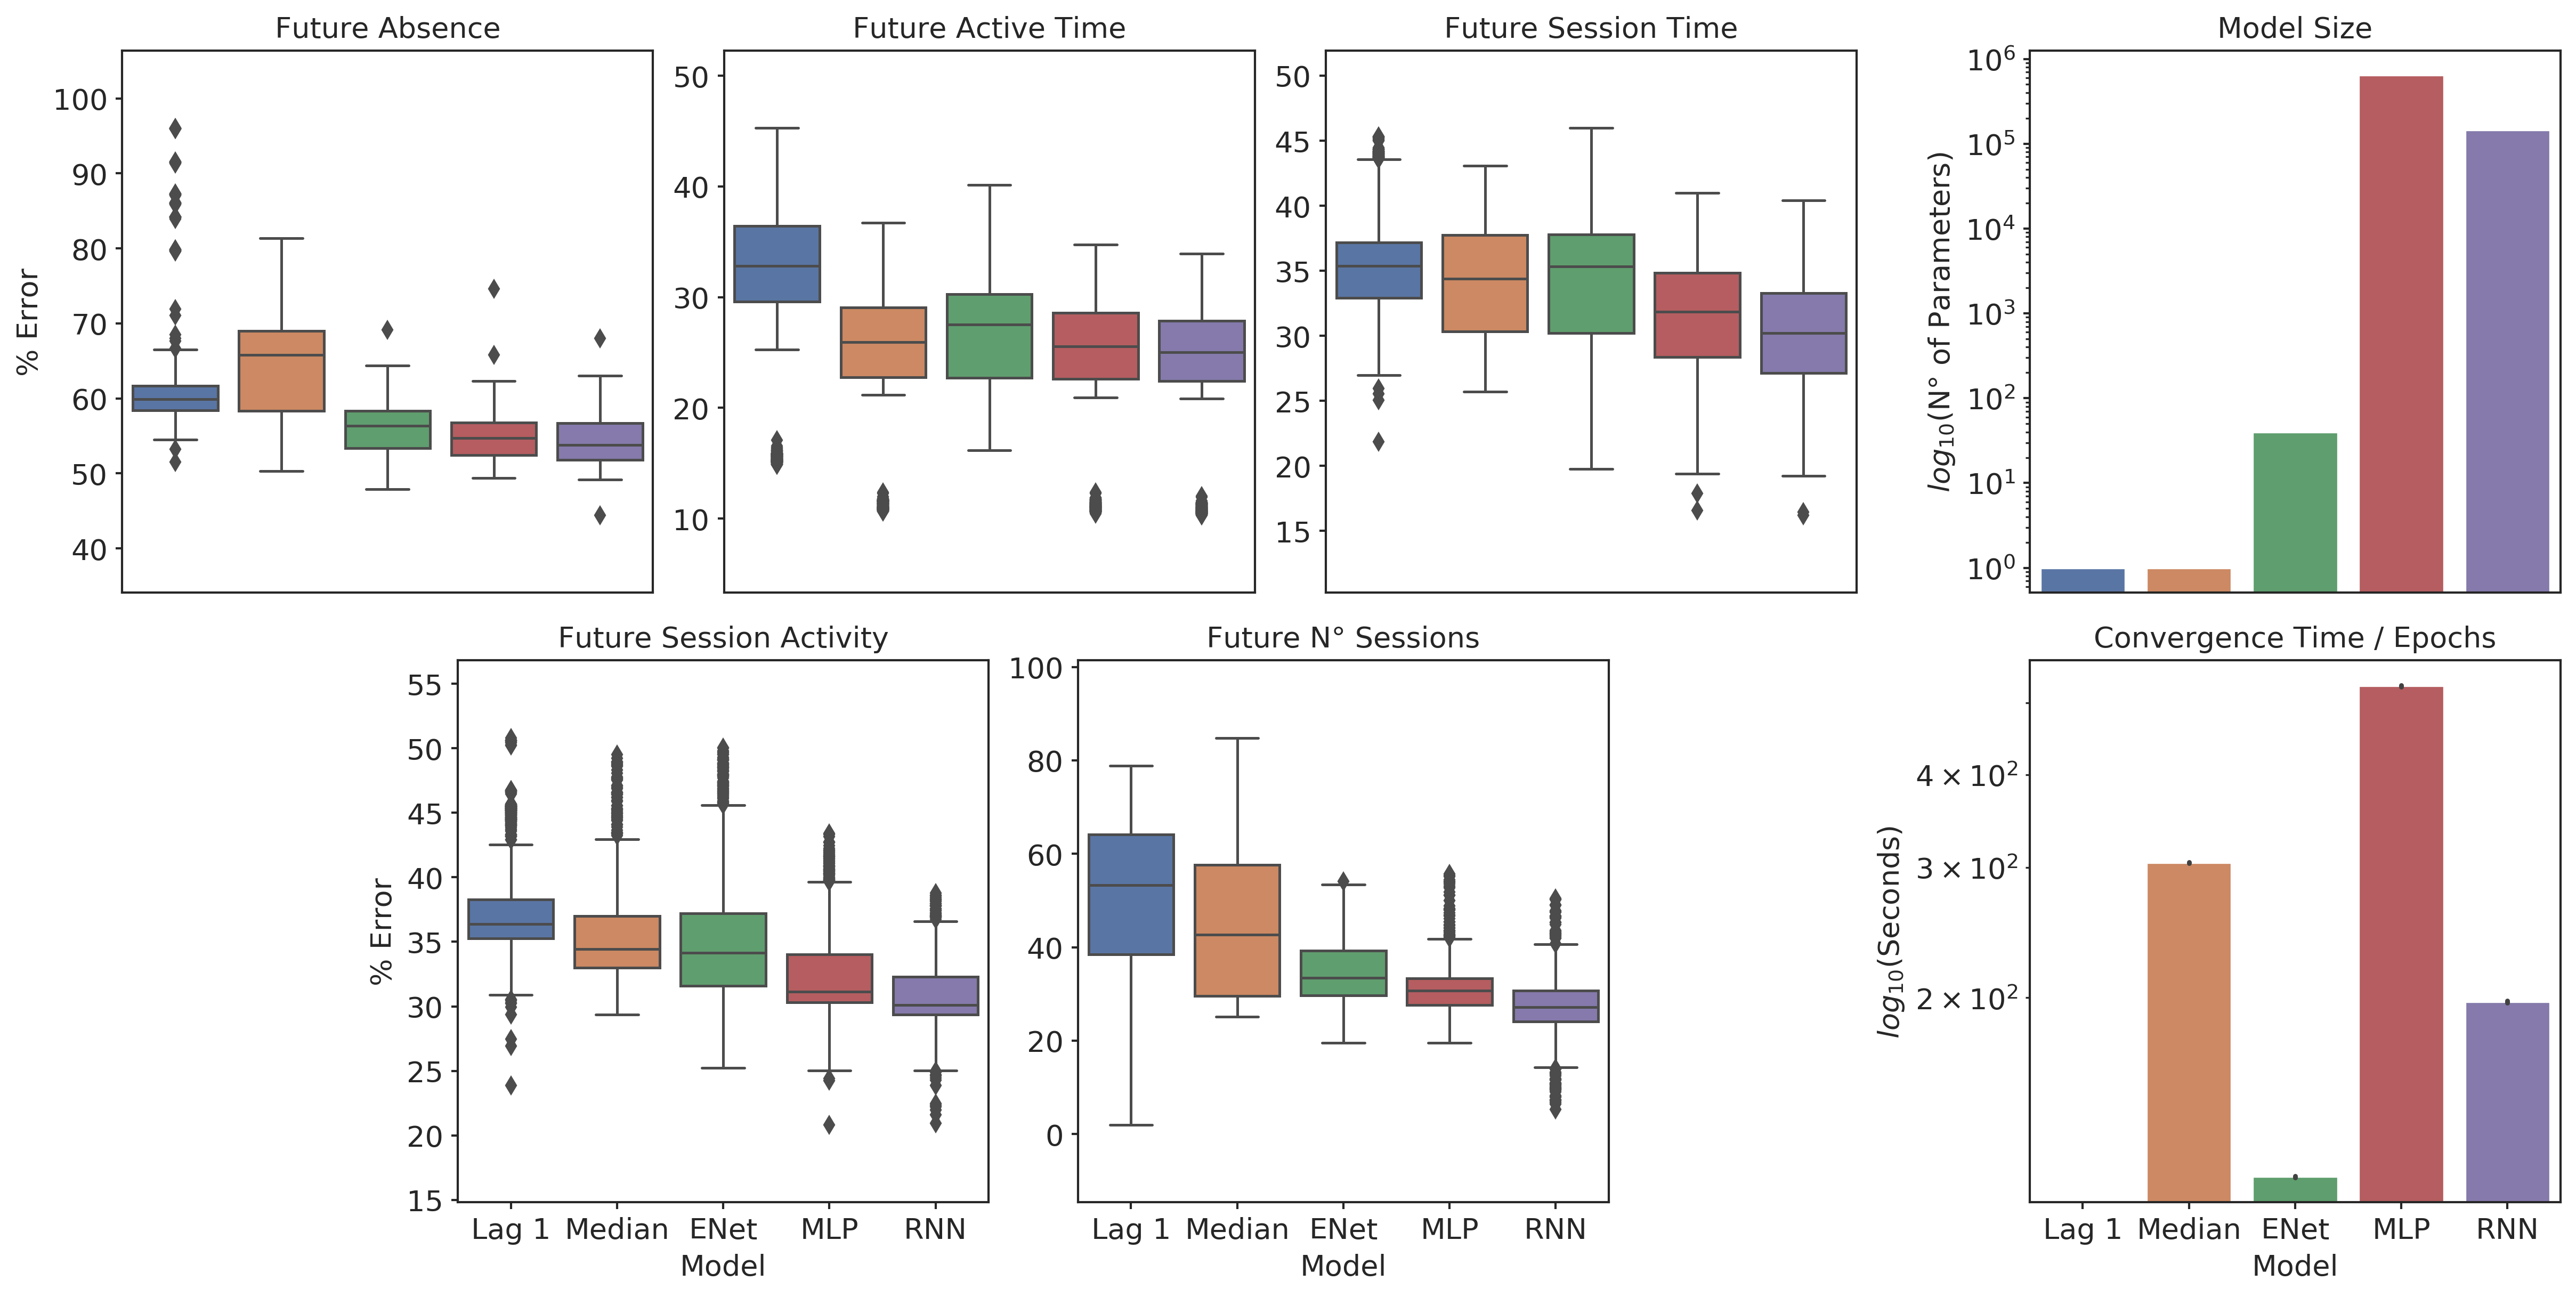
\includegraphics[width=.8\textwidth]{images/chapter_3/performance_exploded_32.png}
\caption{\textbf{Dis-aggregated comparison of models' performance.}. Our approach (RNN) outperformed all competing ones on each target. It consistently used fewer parameters and had shorter computation time than the second best performing model. Box-plots show the 10-fold cross-validation performance expressed as percentage of error (i.e. SMAPE) of each model for the five targets. The bar-plot on the top row indicates the number of free parameters for each model while the bar plot on the bottom row shows the average time for each training epoch. Both bar-plots are $log_{10}$ scaled.}
\label{model_comp_non_coll} 
\end{figure*}

\subsection{Model Criticism}

The advantage provided by the combination of non-linearity and recurrency in the estimation task is in line with the dynamical nature of motivation and incentive salience attribution \cite{toates1994comparing,robinson1993neural,zhang2009neural,tindell2009dynamic,berridge2012prediction}. This is also consistent with a body of research showing that the attribution of value to potentially rewarding objects or actions is often carried out by non-linear recurrent operations \cite{song2017reward,wang2018prefrontal} and that Artificial Neural Networks with recurrent connections are well suited for approximating these operations \cite{kietzmann2018deep}. These findings are corroborated not just by the superior performance of the RNN model in the prediction task (see section \ref{perf_results}) but also by its capacity to produce more stable representations (see Figure \ref{predictive_panel}). The work we just presented is not exempt from limitations. Our approach is formally different from that of TD Learning \footnote{See \cite{barto2004reinforcement} for a  review of the differences between supervised and reinforcement learning.} and does not model the process of incentive salience attribution but rather attempt to approximate the product of this process (i.e. changes in attributed incentive salience). For this reason a direct comparison with the work of McClure \textit{et. al.} \cite{mcclure2003computational} and Zhang \textit{et. al.} \cite{zhang2009neural} is difficult. Moreover, unlike TD learning \cite{schultz1997neural} our model is not guaranteed to converge on a quantification of $V$ that is directly comparable to its biological counterpart or that has arisen from the same type of computations. This is also reinforced by the differences in mechanistic functioning between biological and artificial neural networks \cite{lillicrap2019backpropagation,lillicrap2020backpropagation}. These issues are partially attenuated by the constraints provided by our theoretical framework but in line with similar reports in the literature \cite{calhoun2019unsupervised,wang2018prefrontal} a verification based on controlled experiments is desirable. Differently from the works of Calhoun \textit{et. al.} \cite{calhoun2019unsupervised},  McClure \textit{et. al.} \cite{mcclure2003computational} and Zhang \textit{et. al.} \cite{zhang2009neural}, our methodology relies on a  supervised learning approach to perform both prediction of future behaviour and latent state estimation, making this two tasks infeasible before any data is observed. This limitation could be attenuated by initializing our model using a representation  generated in an unsupervised manner. As we mentioned in section \ref{videogame_telemetries} the reward dynamics generated by the interaction between the individual and the game incentive mechanics play an important role in determining the intensity of future playing behaviour \cite{agarwal2017quitting, avserivskis2017computational, wang2018beyond}. In addition to this, we know that these dynamics are modulated by the internal state of the individual \cite{zhang2009neural} and by the context in which in which they are generated \cite{palminteri2015contextual}. These factors, were only partially captured by our approach as they require a higher temporal resolution (i.e. within rather than between sessions) as well as more granular indices (i.e. in-game and environmental information) than those we employed. As a consequence we can see how our approach, despite outperforming competing ones, still achieves a relatively high error rate in predicting some behavioural targets (e.g. future Absence). A possible solution to this would be to incorporate information about the context in which the observed behaviour occurred (e.g. time, location or in-game events) and adapt the architecture of our model accordingly. As well as improving the performance of the model, this should also increase the quality of the generated representation and consequently also that of the derived behavioural profiles. Lastly, despite the fact that our approach appeared to deal gracefully  with objects having different structural characteristics, these were limited to the domain of video games. In order to verify the generalizability of our approach, future work should include data generated from a variety of contexts (e.g. web services, online and laboratory-based experiments).

\section{Dynamic Prediction of Future Behavioural Intensity with Environmental and Game Covariates}
\label{model_architecture_1}
\lorem

\subsection{Model Design}
\begin{figure}[ht]
\begin{center}
\begin{adjustbox}{width=0.7\textwidth}
    \tikzset{every picture/.style={line width=0.75pt}} %set default line width to 0.75pt        
    
    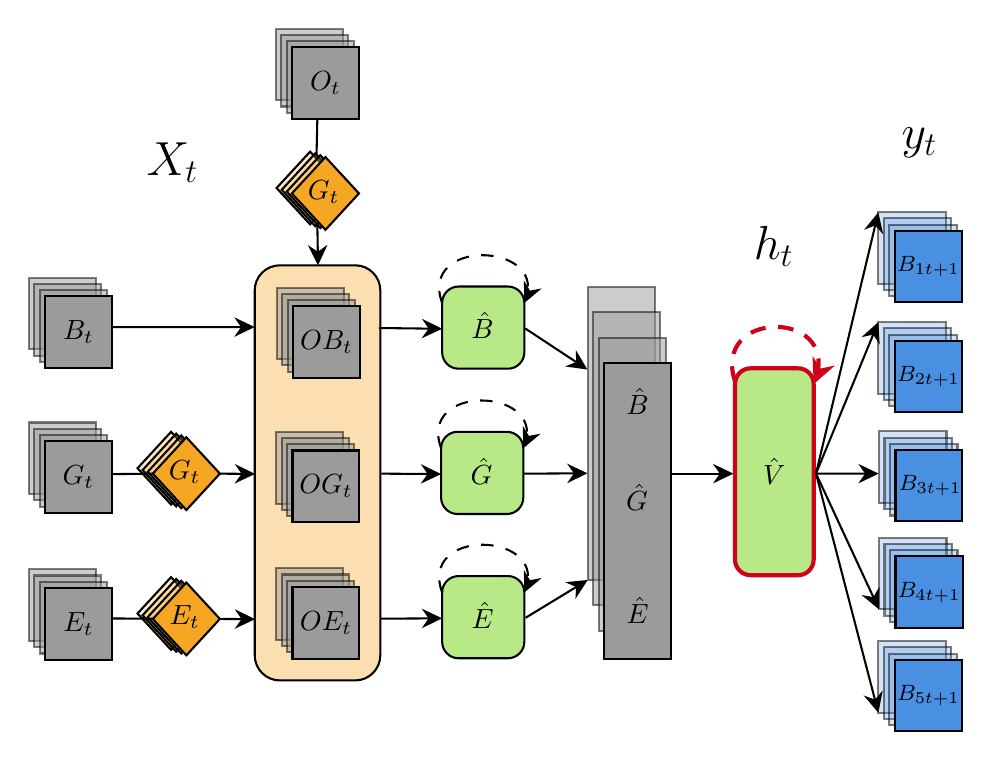
\begin{tikzpicture}[x=0.75pt,y=0.75pt,yscale=-1,xscale=1]
    %uncomment if require: \path (0,411); %set diagram left start at 0, and has height of 411
    
    %Rounded Rect [id:dp15650356150345013] 
    \draw  [fill={rgb, 255:red, 245; green, 166; blue, 35 }  ,fill opacity=0.36 ] (219.9,142.15) .. controls (219.9,135.47) and (225.32,130.05) .. (232,130.05) -- (268.3,130.05) .. controls (274.98,130.05) and (280.4,135.47) .. (280.4,142.15) -- (280.4,317.95) .. controls (280.4,324.63) and (274.98,330.05) .. (268.3,330.05) -- (232,330.05) .. controls (225.32,330.05) and (219.9,324.63) .. (219.9,317.95) -- cycle ;
    %Straight Lines [id:da409284418173784] 
    \draw    (250.06,109.76) -- (250.35,127.05) ;
    \draw [shift={(250.4,130.05)}, rotate = 269.03] [fill={rgb, 255:red, 0; green, 0; blue, 0 }  ][line width=0.08]  [draw opacity=0] (9.82,-4.72) -- (0,0) -- (9.82,4.72) -- (6.52,0) -- cycle    ;
    %Shape: Rectangle [id:dp7034345660290355] 
    \draw  [color={rgb, 255:red, 0; green, 0; blue, 0 }  ,draw opacity=0.5 ][fill={rgb, 255:red, 155; green, 155; blue, 155 }  ,fill opacity=0.5 ] (111.01,276.53) -- (143.26,276.53) -- (143.26,311.05) -- (111.01,311.05) -- cycle ;
    %Shape: Rectangle [id:dp22118233628007533] 
    \draw  [color={rgb, 255:red, 0; green, 0; blue, 0 }  ,draw opacity=0.5 ][fill={rgb, 255:red, 155; green, 155; blue, 155 }  ,fill opacity=0.5 ] (113.63,279.51) -- (145.88,279.51) -- (145.88,314.03) -- (113.63,314.03) -- cycle ;
    %Shape: Rectangle [id:dp24867768000931467] 
    \draw  [color={rgb, 255:red, 0; green, 0; blue, 0 }  ,draw opacity=0.5 ][fill={rgb, 255:red, 155; green, 155; blue, 155 }  ,fill opacity=0.5 ] (116.27,282.56) -- (148.53,282.56) -- (148.53,317.08) -- (116.27,317.08) -- cycle ;
    %Shape: Rectangle [id:dp124905579804508] 
    \draw  [fill={rgb, 255:red, 155; green, 155; blue, 155 }  ,fill opacity=1 ] (118.86,285.5) -- (151.11,285.5) -- (151.11,320.02) -- (118.86,320.02) -- cycle ;
    %Straight Lines [id:da8537240673366849] 
    \draw    (250.06,59.86) -- (249.67,77.43) ;
    %Rounded Rect [id:dp9724403504665806] 
    \draw  [color={rgb, 255:red, 208; green, 2; blue, 27 }  ,draw opacity=1 ][fill={rgb, 255:red, 184; green, 233; blue, 134 }  ,fill opacity=1 ][line width=1.5]  (451.3,187.25) .. controls (451.3,183.06) and (454.7,179.67) .. (458.88,179.67) -- (481.62,179.67) .. controls (485.81,179.67) and (489.2,183.06) .. (489.2,187.25) -- (489.2,271.79) .. controls (489.2,275.97) and (485.81,279.37) .. (481.62,279.37) -- (458.88,279.37) .. controls (454.7,279.37) and (451.3,275.97) .. (451.3,271.79) -- cycle ;
    %Curve Lines [id:da6973720397061056] 
    \draw [color={rgb, 255:red, 208; green, 2; blue, 27 }  ,draw opacity=1 ][line width=1.5]  [dash pattern={on 5.63pt off 4.5pt}]  (451.3,186.02) .. controls (439.95,151.4) and (500.2,151.33) .. (490.53,183.61) ;
    \draw [shift={(489.2,187.25)}, rotate = 293.32] [fill={rgb, 255:red, 208; green, 2; blue, 27 }  ,fill opacity=1 ][line width=0.08]  [draw opacity=0] (12.23,-5.88) -- (0,0) -- (12.23,5.88) -- (8.12,0) -- cycle    ;
    %Shape: Rectangle [id:dp1958055080757597] 
    \draw  [color={rgb, 255:red, 0; green, 0; blue, 0 }  ,draw opacity=0.5 ][fill={rgb, 255:red, 74; green, 144; blue, 226 }  ,fill opacity=0.25 ] (520.36,157.39) -- (552.87,157.39) -- (552.87,191.9) -- (520.36,191.9) -- cycle ;
    %Shape: Rectangle [id:dp20825701586292622] 
    \draw  [color={rgb, 255:red, 0; green, 0; blue, 0 }  ,draw opacity=0.5 ][fill={rgb, 255:red, 74; green, 144; blue, 226 }  ,fill opacity=0.25 ] (523,160.37) -- (555.51,160.37) -- (555.51,194.88) -- (523,194.88) -- cycle ;
    %Shape: Rectangle [id:dp6709034910590727] 
    \draw  [color={rgb, 255:red, 0; green, 0; blue, 0 }  ,draw opacity=0.5 ][fill={rgb, 255:red, 74; green, 144; blue, 226 }  ,fill opacity=0.25 ] (525.67,163.42) -- (558.17,163.42) -- (558.17,197.93) -- (525.67,197.93) -- cycle ;
    %Shape: Rectangle [id:dp943426610209301] 
    \draw  [fill={rgb, 255:red, 74; green, 144; blue, 226 }  ,fill opacity=1 ] (528.28,166.36) -- (560.78,166.36) -- (560.78,200.87) -- (528.28,200.87) -- cycle ;
    %Shape: Rectangle [id:dp9270730461824767] 
    \draw  [color={rgb, 255:red, 0; green, 0; blue, 0 }  ,draw opacity=0.5 ][fill={rgb, 255:red, 74; green, 144; blue, 226 }  ,fill opacity=0.25 ] (520.69,210.06) -- (553.2,210.06) -- (553.2,244.56) -- (520.69,244.56) -- cycle ;
    %Shape: Rectangle [id:dp9671567967621458] 
    \draw  [color={rgb, 255:red, 0; green, 0; blue, 0 }  ,draw opacity=0.5 ][fill={rgb, 255:red, 74; green, 144; blue, 226 }  ,fill opacity=0.25 ] (523.33,213.04) -- (555.84,213.04) -- (555.84,247.54) -- (523.33,247.54) -- cycle ;
    %Shape: Rectangle [id:dp6567850092606636] 
    \draw  [color={rgb, 255:red, 0; green, 0; blue, 0 }  ,draw opacity=0.5 ][fill={rgb, 255:red, 74; green, 144; blue, 226 }  ,fill opacity=0.25 ] (526,216.09) -- (558.5,216.09) -- (558.5,250.6) -- (526,250.6) -- cycle ;
    %Shape: Rectangle [id:dp9307909660529495] 
    \draw  [fill={rgb, 255:red, 74; green, 144; blue, 226 }  ,fill opacity=1 ] (528.62,219.02) -- (560.84,219.02) -- (560.84,253.22) -- (528.62,253.22) -- cycle ;
    %Shape: Rectangle [id:dp2956426995252315] 
    \draw  [color={rgb, 255:red, 0; green, 0; blue, 0 }  ,draw opacity=0.5 ][fill={rgb, 255:red, 74; green, 144; blue, 226 }  ,fill opacity=0.25 ] (520.36,311.11) -- (552.87,311.11) -- (552.87,345.62) -- (520.36,345.62) -- cycle ;
    %Shape: Rectangle [id:dp9676718309145981] 
    \draw  [color={rgb, 255:red, 0; green, 0; blue, 0 }  ,draw opacity=0.5 ][fill={rgb, 255:red, 74; green, 144; blue, 226 }  ,fill opacity=0.25 ] (523,314.09) -- (555.51,314.09) -- (555.51,348.6) -- (523,348.6) -- cycle ;
    %Shape: Rectangle [id:dp3802447939611997] 
    \draw  [color={rgb, 255:red, 0; green, 0; blue, 0 }  ,draw opacity=0.5 ][fill={rgb, 255:red, 74; green, 144; blue, 226 }  ,fill opacity=0.25 ] (525.67,317.14) -- (558.17,317.14) -- (558.17,351.65) -- (525.67,351.65) -- cycle ;
    %Shape: Rectangle [id:dp2655409211543931] 
    \draw  [fill={rgb, 255:red, 74; green, 144; blue, 226 }  ,fill opacity=1 ] (528.28,320.08) -- (560.78,320.08) -- (560.78,354.59) -- (528.28,354.59) -- cycle ;
    %Shape: Rectangle [id:dp4040153422296009] 
    \draw  [color={rgb, 255:red, 0; green, 0; blue, 0 }  ,draw opacity=0.5 ][fill={rgb, 255:red, 74; green, 144; blue, 226 }  ,fill opacity=0.25 ] (520.69,261.32) -- (553.2,261.32) -- (553.2,295.83) -- (520.69,295.83) -- cycle ;
    %Shape: Rectangle [id:dp7066102537923638] 
    \draw  [color={rgb, 255:red, 0; green, 0; blue, 0 }  ,draw opacity=0.5 ][fill={rgb, 255:red, 74; green, 144; blue, 226 }  ,fill opacity=0.25 ] (523.33,264.3) -- (555.84,264.3) -- (555.84,298.81) -- (523.33,298.81) -- cycle ;
    %Shape: Rectangle [id:dp46050637304135866] 
    \draw  [color={rgb, 255:red, 0; green, 0; blue, 0 }  ,draw opacity=0.5 ][fill={rgb, 255:red, 74; green, 144; blue, 226 }  ,fill opacity=0.25 ] (526,267.35) -- (558.5,267.35) -- (558.5,301.86) -- (526,301.86) -- cycle ;
    %Shape: Rectangle [id:dp2033829273595421] 
    \draw  [fill={rgb, 255:red, 74; green, 144; blue, 226 }  ,fill opacity=1 ] (528.61,270.29) -- (561.11,270.29) -- (561.11,304.8) -- (528.61,304.8) -- cycle ;
    %Shape: Rectangle [id:dp19424752965877823] 
    \draw  [color={rgb, 255:red, 0; green, 0; blue, 0 }  ,draw opacity=0.5 ][fill={rgb, 255:red, 74; green, 144; blue, 226 }  ,fill opacity=0.25 ] (520.36,104.48) -- (552.87,104.48) -- (552.87,138.98) -- (520.36,138.98) -- cycle ;
    %Shape: Rectangle [id:dp6987771152166413] 
    \draw  [color={rgb, 255:red, 0; green, 0; blue, 0 }  ,draw opacity=0.5 ][fill={rgb, 255:red, 74; green, 144; blue, 226 }  ,fill opacity=0.25 ] (523,107.46) -- (555.51,107.46) -- (555.51,141.96) -- (523,141.96) -- cycle ;
    %Shape: Rectangle [id:dp12765942569283661] 
    \draw  [color={rgb, 255:red, 0; green, 0; blue, 0 }  ,draw opacity=0.5 ][fill={rgb, 255:red, 74; green, 144; blue, 226 }  ,fill opacity=0.25 ] (525.67,110.51) -- (558.17,110.51) -- (558.17,145.01) -- (525.67,145.01) -- cycle ;
    %Shape: Rectangle [id:dp16248810139444148] 
    \draw  [fill={rgb, 255:red, 74; green, 144; blue, 226 }  ,fill opacity=1 ] (528.28,113.44) -- (560.78,113.44) -- (560.78,147.95) -- (528.28,147.95) -- cycle ;
    %Shape: Rectangle [id:dp7988673729176894] 
    \draw  [color={rgb, 255:red, 0; green, 0; blue, 0 }  ,draw opacity=0.5 ][fill={rgb, 255:red, 155; green, 155; blue, 155 }  ,fill opacity=0.5 ] (111.01,205.77) -- (143.26,205.77) -- (143.26,240.29) -- (111.01,240.29) -- cycle ;
    %Shape: Rectangle [id:dp9623129937085917] 
    \draw  [color={rgb, 255:red, 0; green, 0; blue, 0 }  ,draw opacity=0.5 ][fill={rgb, 255:red, 155; green, 155; blue, 155 }  ,fill opacity=0.5 ] (113.63,208.75) -- (145.88,208.75) -- (145.88,243.27) -- (113.63,243.27) -- cycle ;
    %Shape: Rectangle [id:dp429379441325212] 
    \draw  [color={rgb, 255:red, 0; green, 0; blue, 0 }  ,draw opacity=0.5 ][fill={rgb, 255:red, 155; green, 155; blue, 155 }  ,fill opacity=0.5 ] (116.27,211.8) -- (148.53,211.8) -- (148.53,246.32) -- (116.27,246.32) -- cycle ;
    %Shape: Rectangle [id:dp9493890675957639] 
    \draw  [fill={rgb, 255:red, 155; green, 155; blue, 155 }  ,fill opacity=1 ] (118.86,214.74) -- (151.11,214.74) -- (151.11,249.26) -- (118.86,249.26) -- cycle ;
    %Straight Lines [id:da0399560958706785] 
    \draw [fill={rgb, 255:red, 155; green, 155; blue, 155 }  ,fill opacity=1 ]   (150.09,159.83) -- (216.85,159.8) ;
    \draw [shift={(219.85,159.8)}, rotate = 179.98] [fill={rgb, 255:red, 0; green, 0; blue, 0 }  ][line width=0.08]  [draw opacity=0] (9.82,-4.72) -- (0,0) -- (9.82,4.72) -- (6.52,0) -- cycle    ;
    %Shape: Rectangle [id:dp3393145890474042] 
    \draw  [color={rgb, 255:red, 0; green, 0; blue, 0 }  ,draw opacity=0.5 ][fill={rgb, 255:red, 155; green, 155; blue, 155 }  ,fill opacity=0.5 ] (111.01,136.06) -- (143.26,136.06) -- (143.26,170.57) -- (111.01,170.57) -- cycle ;
    %Shape: Rectangle [id:dp27631704382885136] 
    \draw  [color={rgb, 255:red, 0; green, 0; blue, 0 }  ,draw opacity=0.5 ][fill={rgb, 255:red, 155; green, 155; blue, 155 }  ,fill opacity=0.5 ] (113.63,139.04) -- (145.88,139.04) -- (145.88,173.55) -- (113.63,173.55) -- cycle ;
    %Shape: Rectangle [id:dp8553441662393909] 
    \draw  [color={rgb, 255:red, 0; green, 0; blue, 0 }  ,draw opacity=0.5 ][fill={rgb, 255:red, 155; green, 155; blue, 155 }  ,fill opacity=0.5 ] (116.27,142.09) -- (148.53,142.09) -- (148.53,176.61) -- (116.27,176.61) -- cycle ;
    %Shape: Rectangle [id:dp4571491350911555] 
    \draw  [fill={rgb, 255:red, 155; green, 155; blue, 155 }  ,fill opacity=1 ] (118.86,145.03) -- (151.11,145.03) -- (151.11,179.54) -- (118.86,179.54) -- cycle ;
    %Shape: Diamond [id:dp42134346339770745] 
    \draw  [fill={rgb, 255:red, 245; green, 166; blue, 35 }  ,fill opacity=0.25 ] (179.6,210.28) -- (195.77,227.81) -- (179.6,245.33) -- (163.43,227.81) -- cycle ;
    %Shape: Diamond [id:dp8160874162123375] 
    \draw  [fill={rgb, 255:red, 245; green, 166; blue, 35 }  ,fill opacity=0.25 ] (182.05,211.16) -- (198.22,228.68) -- (182.05,246.2) -- (165.89,228.68) -- cycle ;
    %Shape: Diamond [id:dp05986250472128074] 
    \draw  [fill={rgb, 255:red, 245; green, 166; blue, 35 }  ,fill opacity=0.25 ] (184.51,212.04) -- (200.68,229.56) -- (184.51,247.08) -- (168.34,229.56) -- cycle ;
    %Shape: Diamond [id:dp6831575900746938] 
    \draw  [fill={rgb, 255:red, 245; green, 166; blue, 35 }  ,fill opacity=1 ] (186.97,212.91) -- (203.13,230.43) -- (186.97,247.96) -- (170.8,230.43) -- cycle ;
    %Straight Lines [id:da3169233008507637] 
    \draw    (151.46,230.66) -- (170.8,230.43) ;
    %Shape: Diamond [id:dp08100159339963764] 
    \draw  [fill={rgb, 255:red, 245; green, 166; blue, 35 }  ,fill opacity=0.25 ] (179.6,280.28) -- (195.77,297.81) -- (179.6,315.33) -- (163.43,297.81) -- cycle ;
    %Shape: Diamond [id:dp6545409040088919] 
    \draw  [fill={rgb, 255:red, 245; green, 166; blue, 35 }  ,fill opacity=0.25 ] (182.05,281.16) -- (198.22,298.68) -- (182.05,316.2) -- (165.89,298.68) -- cycle ;
    %Shape: Diamond [id:dp22008618792927115] 
    \draw  [fill={rgb, 255:red, 245; green, 166; blue, 35 }  ,fill opacity=0.25 ] (184.51,282.04) -- (200.68,299.56) -- (184.51,317.08) -- (168.34,299.56) -- cycle ;
    %Shape: Diamond [id:dp6216162169932065] 
    \draw  [fill={rgb, 255:red, 245; green, 166; blue, 35 }  ,fill opacity=1 ] (186.97,282.91) -- (203.13,300.43) -- (186.97,317.96) -- (170.8,300.43) -- cycle ;
    %Straight Lines [id:da6348314705630924] 
    \draw    (203.13,300.43) -- (217.07,300.51) ;
    \draw [shift={(220.07,300.53)}, rotate = 180.32] [fill={rgb, 255:red, 0; green, 0; blue, 0 }  ][line width=0.08]  [draw opacity=0] (9.82,-4.72) -- (0,0) -- (9.82,4.72) -- (6.52,0) -- cycle    ;
    %Straight Lines [id:da29443986089740126] 
    \draw    (150.89,300.2) -- (170.89,300.31) ;
    %Straight Lines [id:da7037674707293678] 
    \draw [fill={rgb, 255:red, 155; green, 155; blue, 155 }  ,fill opacity=1 ]   (279.77,160.26) -- (307.2,160.6) ;
    \draw [shift={(310.2,160.63)}, rotate = 180.71] [fill={rgb, 255:red, 0; green, 0; blue, 0 }  ][line width=0.08]  [draw opacity=0] (9.82,-4.72) -- (0,0) -- (9.82,4.72) -- (6.52,0) -- cycle    ;
    %Rounded Rect [id:dp05798817292021641] 
    \draw  [color={rgb, 255:red, 0; green, 0; blue, 0 }  ,draw opacity=1 ][fill={rgb, 255:red, 184; green, 233; blue, 134 }  ,fill opacity=1 ][line width=0.75]  (310.2,148.19) .. controls (310.2,143.81) and (313.75,140.27) .. (318.12,140.27) -- (341.88,140.27) .. controls (346.25,140.27) and (349.8,143.81) .. (349.8,148.19) -- (349.8,171.95) .. controls (349.8,176.32) and (346.25,179.87) .. (341.88,179.87) -- (318.12,179.87) .. controls (313.75,179.87) and (310.2,176.32) .. (310.2,171.95) -- cycle ;
    %Curve Lines [id:da04021743223527896] 
    \draw [color={rgb, 255:red, 0; green, 0; blue, 0 }  ,draw opacity=1 ][line width=0.75]  [dash pattern={on 4.5pt off 4.5pt}]  (310.2,148.19) .. controls (298.92,117.06) and (359.25,118.81) .. (350.79,145.63) ;
    \draw [shift={(349.8,148.19)}, rotate = 294.37] [fill={rgb, 255:red, 0; green, 0; blue, 0 }  ,fill opacity=1 ][line width=0.08]  [draw opacity=0] (9.82,-4.72) -- (0,0) -- (9.82,4.72) -- (6.52,0) -- cycle    ;
    %Straight Lines [id:da04725287763752273] 
    \draw [fill={rgb, 255:red, 155; green, 155; blue, 155 }  ,fill opacity=1 ]   (350.2,160.45) -- (377.7,178.6) ;
    \draw [shift={(380.2,180.25)}, rotate = 213.42] [fill={rgb, 255:red, 0; green, 0; blue, 0 }  ][line width=0.08]  [draw opacity=0] (9.82,-4.72) -- (0,0) -- (9.82,4.72) -- (6.52,0) -- cycle    ;
    %Straight Lines [id:da6945773359077246] 
    \draw    (203.13,230.43) -- (217.07,230.54) ;
    \draw [shift={(220.07,230.56)}, rotate = 180.44] [fill={rgb, 255:red, 0; green, 0; blue, 0 }  ][line width=0.08]  [draw opacity=0] (9.82,-4.72) -- (0,0) -- (9.82,4.72) -- (6.52,0) -- cycle    ;
    %Straight Lines [id:da6273046628189572] 
    \draw [fill={rgb, 255:red, 155; green, 155; blue, 155 }  ,fill opacity=1 ]   (280.91,230.43) -- (306.7,230.61) ;
    \draw [shift={(309.7,230.63)}, rotate = 180.41] [fill={rgb, 255:red, 0; green, 0; blue, 0 }  ][line width=0.08]  [draw opacity=0] (9.82,-4.72) -- (0,0) -- (9.82,4.72) -- (6.52,0) -- cycle    ;
    %Rounded Rect [id:dp7958241287205053] 
    \draw  [color={rgb, 255:red, 0; green, 0; blue, 0 }  ,draw opacity=1 ][fill={rgb, 255:red, 184; green, 233; blue, 134 }  ,fill opacity=1 ][line width=0.75]  (309.7,218.19) .. controls (309.7,213.81) and (313.25,210.27) .. (317.62,210.27) -- (341.38,210.27) .. controls (345.75,210.27) and (349.3,213.81) .. (349.3,218.19) -- (349.3,241.95) .. controls (349.3,246.32) and (345.75,249.87) .. (341.38,249.87) -- (317.62,249.87) .. controls (313.25,249.87) and (309.7,246.32) .. (309.7,241.95) -- cycle ;
    %Curve Lines [id:da19079237969225638] 
    \draw [color={rgb, 255:red, 0; green, 0; blue, 0 }  ,draw opacity=1 ][line width=0.75]  [dash pattern={on 4.5pt off 4.5pt}]  (309.7,218.19) .. controls (298.42,187.06) and (358.75,188.81) .. (350.29,215.63) ;
    \draw [shift={(349.3,218.19)}, rotate = 294.37] [fill={rgb, 255:red, 0; green, 0; blue, 0 }  ,fill opacity=1 ][line width=0.08]  [draw opacity=0] (9.82,-4.72) -- (0,0) -- (9.82,4.72) -- (6.52,0) -- cycle    ;
    %Straight Lines [id:da5724582303552335] 
    \draw [fill={rgb, 255:red, 155; green, 155; blue, 155 }  ,fill opacity=1 ]   (280.63,300.31) -- (307.2,300.15) ;
    \draw [shift={(310.2,300.13)}, rotate = 179.65] [fill={rgb, 255:red, 0; green, 0; blue, 0 }  ][line width=0.08]  [draw opacity=0] (9.82,-4.72) -- (0,0) -- (9.82,4.72) -- (6.52,0) -- cycle    ;
    %Rounded Rect [id:dp6456487678445413] 
    \draw  [color={rgb, 255:red, 0; green, 0; blue, 0 }  ,draw opacity=1 ][fill={rgb, 255:red, 184; green, 233; blue, 134 }  ,fill opacity=1 ][line width=0.75]  (310.2,287.69) .. controls (310.2,283.31) and (313.75,279.77) .. (318.12,279.77) -- (341.88,279.77) .. controls (346.25,279.77) and (349.8,283.31) .. (349.8,287.69) -- (349.8,311.45) .. controls (349.8,315.82) and (346.25,319.37) .. (341.88,319.37) -- (318.12,319.37) .. controls (313.75,319.37) and (310.2,315.82) .. (310.2,311.45) -- cycle ;
    %Curve Lines [id:da6374705672660576] 
    \draw [color={rgb, 255:red, 0; green, 0; blue, 0 }  ,draw opacity=1 ][line width=0.75]  [dash pattern={on 4.5pt off 4.5pt}]  (310.2,287.69) .. controls (298.92,256.56) and (359.25,258.31) .. (350.79,285.13) ;
    \draw [shift={(349.8,287.69)}, rotate = 294.37] [fill={rgb, 255:red, 0; green, 0; blue, 0 }  ,fill opacity=1 ][line width=0.08]  [draw opacity=0] (9.82,-4.72) -- (0,0) -- (9.82,4.72) -- (6.52,0) -- cycle    ;
    %Shape: Rectangle [id:dp53907172122875] 
    \draw  [color={rgb, 255:red, 0; green, 0; blue, 0 }  ,draw opacity=0.5 ][fill={rgb, 255:red, 155; green, 155; blue, 155 }  ,fill opacity=0.5 ] (230.01,16.06) -- (262.26,16.06) -- (262.26,50.57) -- (230.01,50.57) -- cycle ;
    %Shape: Rectangle [id:dp009192212091793661] 
    \draw  [color={rgb, 255:red, 0; green, 0; blue, 0 }  ,draw opacity=0.5 ][fill={rgb, 255:red, 155; green, 155; blue, 155 }  ,fill opacity=0.5 ] (232.63,19.04) -- (264.88,19.04) -- (264.88,53.55) -- (232.63,53.55) -- cycle ;
    %Shape: Rectangle [id:dp10982806096562447] 
    \draw  [color={rgb, 255:red, 0; green, 0; blue, 0 }  ,draw opacity=0.5 ][fill={rgb, 255:red, 155; green, 155; blue, 155 }  ,fill opacity=0.5 ] (235.27,22.09) -- (267.53,22.09) -- (267.53,56.61) -- (235.27,56.61) -- cycle ;
    %Shape: Rectangle [id:dp024787601372134982] 
    \draw  [fill={rgb, 255:red, 155; green, 155; blue, 155 }  ,fill opacity=1 ] (237.86,25.03) -- (270.11,25.03) -- (270.11,59.54) -- (237.86,59.54) -- cycle ;
    %Shape: Rectangle [id:dp9022114030928725] 
    \draw  [color={rgb, 255:red, 0; green, 0; blue, 0 }  ,draw opacity=0.5 ][fill={rgb, 255:red, 155; green, 155; blue, 155 }  ,fill opacity=0.5 ] (380.34,140.45) -- (412.6,140.45) -- (412.6,281.66) -- (380.34,281.66) -- cycle ;
    %Shape: Rectangle [id:dp9877830883323443] 
    \draw  [color={rgb, 255:red, 0; green, 0; blue, 0 }  ,draw opacity=0.5 ][fill={rgb, 255:red, 155; green, 155; blue, 155 }  ,fill opacity=0.5 ] (382.96,152.64) -- (415.22,152.64) -- (415.22,293.84) -- (382.96,293.84) -- cycle ;
    %Shape: Rectangle [id:dp8814167498359042] 
    \draw  [color={rgb, 255:red, 0; green, 0; blue, 0 }  ,draw opacity=0.5 ][fill={rgb, 255:red, 155; green, 155; blue, 155 }  ,fill opacity=0.5 ] (385.61,165.13) -- (417.86,165.13) -- (417.86,306.34) -- (385.61,306.34) -- cycle ;
    %Shape: Rectangle [id:dp5289911737134959] 
    \draw  [fill={rgb, 255:red, 155; green, 155; blue, 155 }  ,fill opacity=1 ] (388.19,177.14) -- (420.45,177.14) -- (420.45,319.53) -- (388.19,319.53) -- cycle ;
    %Shape: Rectangle [id:dp8149328215662492] 
    \draw  [color={rgb, 255:red, 0; green, 0; blue, 0 }  ,draw opacity=0.5 ][fill={rgb, 255:red, 155; green, 155; blue, 155 }  ,fill opacity=0.5 ] (230.51,140.77) -- (262.76,140.77) -- (262.76,175.29) -- (230.51,175.29) -- cycle ;
    %Shape: Rectangle [id:dp45921305478843055] 
    \draw  [color={rgb, 255:red, 0; green, 0; blue, 0 }  ,draw opacity=0.5 ][fill={rgb, 255:red, 155; green, 155; blue, 155 }  ,fill opacity=0.5 ] (233.13,143.75) -- (265.38,143.75) -- (265.38,178.27) -- (233.13,178.27) -- cycle ;
    %Shape: Rectangle [id:dp6228279530655318] 
    \draw  [color={rgb, 255:red, 0; green, 0; blue, 0 }  ,draw opacity=0.5 ][fill={rgb, 255:red, 155; green, 155; blue, 155 }  ,fill opacity=0.5 ] (235.77,146.8) -- (268.03,146.8) -- (268.03,181.32) -- (235.77,181.32) -- cycle ;
    %Shape: Rectangle [id:dp3598797805540589] 
    \draw  [fill={rgb, 255:red, 155; green, 155; blue, 155 }  ,fill opacity=1 ] (238.36,149.74) -- (270.61,149.74) -- (270.61,184.26) -- (238.36,184.26) -- cycle ;
    %Shape: Rectangle [id:dp9661891091990619] 
    \draw  [color={rgb, 255:red, 0; green, 0; blue, 0 }  ,draw opacity=0.5 ][fill={rgb, 255:red, 155; green, 155; blue, 155 }  ,fill opacity=0.5 ] (230.26,210.32) -- (262.51,210.32) -- (262.51,244.84) -- (230.26,244.84) -- cycle ;
    %Shape: Rectangle [id:dp690231151268716] 
    \draw  [color={rgb, 255:red, 0; green, 0; blue, 0 }  ,draw opacity=0.5 ][fill={rgb, 255:red, 155; green, 155; blue, 155 }  ,fill opacity=0.5 ] (232.88,213.3) -- (265.13,213.3) -- (265.13,247.82) -- (232.88,247.82) -- cycle ;
    %Shape: Rectangle [id:dp48804619093484347] 
    \draw  [color={rgb, 255:red, 0; green, 0; blue, 0 }  ,draw opacity=0.5 ][fill={rgb, 255:red, 155; green, 155; blue, 155 }  ,fill opacity=0.5 ] (235.52,216.35) -- (267.78,216.35) -- (267.78,250.87) -- (235.52,250.87) -- cycle ;
    %Shape: Rectangle [id:dp22992925838286216] 
    \draw  [fill={rgb, 255:red, 155; green, 155; blue, 155 }  ,fill opacity=1 ] (238.11,219.29) -- (270.36,219.29) -- (270.36,253.81) -- (238.11,253.81) -- cycle ;
    %Shape: Rectangle [id:dp29039742489844134] 
    \draw  [color={rgb, 255:red, 0; green, 0; blue, 0 }  ,draw opacity=0.5 ][fill={rgb, 255:red, 155; green, 155; blue, 155 }  ,fill opacity=0.5 ] (230.26,276.02) -- (262.51,276.02) -- (262.51,310.54) -- (230.26,310.54) -- cycle ;
    %Shape: Rectangle [id:dp42091335353816794] 
    \draw  [color={rgb, 255:red, 0; green, 0; blue, 0 }  ,draw opacity=0.5 ][fill={rgb, 255:red, 155; green, 155; blue, 155 }  ,fill opacity=0.5 ] (232.88,279) -- (265.13,279) -- (265.13,313.52) -- (232.88,313.52) -- cycle ;
    %Shape: Rectangle [id:dp9855473947081604] 
    \draw  [color={rgb, 255:red, 0; green, 0; blue, 0 }  ,draw opacity=0.5 ][fill={rgb, 255:red, 155; green, 155; blue, 155 }  ,fill opacity=0.5 ] (235.52,282.05) -- (267.78,282.05) -- (267.78,316.57) -- (235.52,316.57) -- cycle ;
    %Shape: Rectangle [id:dp434232717458334] 
    \draw  [fill={rgb, 255:red, 155; green, 155; blue, 155 }  ,fill opacity=1 ] (238.11,284.99) -- (270.36,284.99) -- (270.36,319.51) -- (238.11,319.51) -- cycle ;
    %Shape: Diamond [id:dp30872576312410427] 
    \draw  [fill={rgb, 255:red, 245; green, 166; blue, 35 }  ,fill opacity=0.25 ] (246.6,75.28) -- (262.77,92.81) -- (246.6,110.33) -- (230.43,92.81) -- cycle ;
    %Shape: Diamond [id:dp6849972388912634] 
    \draw  [fill={rgb, 255:red, 245; green, 166; blue, 35 }  ,fill opacity=0.25 ] (249.05,76.16) -- (265.22,93.68) -- (249.05,111.2) -- (232.89,93.68) -- cycle ;
    %Shape: Diamond [id:dp857485897511279] 
    \draw  [fill={rgb, 255:red, 245; green, 166; blue, 35 }  ,fill opacity=0.25 ] (251.51,77.04) -- (267.68,94.56) -- (251.51,112.08) -- (235.34,94.56) -- cycle ;
    %Shape: Diamond [id:dp49326046176048577] 
    \draw  [fill={rgb, 255:red, 245; green, 166; blue, 35 }  ,fill opacity=1 ] (253.97,77.91) -- (270.13,95.43) -- (253.97,112.96) -- (237.8,95.43) -- cycle ;
    %Straight Lines [id:da9533396825264671] 
    \draw [fill={rgb, 255:red, 155; green, 155; blue, 155 }  ,fill opacity=1 ]   (349.2,230.45) -- (377.2,230.27) ;
    \draw [shift={(380.2,230.25)}, rotate = 179.63] [fill={rgb, 255:red, 0; green, 0; blue, 0 }  ][line width=0.08]  [draw opacity=0] (9.82,-4.72) -- (0,0) -- (9.82,4.72) -- (6.52,0) -- cycle    ;
    %Straight Lines [id:da46693829157920863] 
    \draw [fill={rgb, 255:red, 155; green, 155; blue, 155 }  ,fill opacity=1 ]   (350.4,299.88) -- (377.78,283.22) ;
    \draw [shift={(380.34,281.66)}, rotate = 148.68] [fill={rgb, 255:red, 0; green, 0; blue, 0 }  ][line width=0.08]  [draw opacity=0] (9.82,-4.72) -- (0,0) -- (9.82,4.72) -- (6.52,0) -- cycle    ;
    %Straight Lines [id:da9477168442608538] 
    \draw [fill={rgb, 255:red, 155; green, 155; blue, 155 }  ,fill opacity=1 ]   (421.09,230.43) -- (447.51,230.43) ;
    \draw [shift={(450.51,230.43)}, rotate = 180] [fill={rgb, 255:red, 0; green, 0; blue, 0 }  ][line width=0.08]  [draw opacity=0] (9.82,-4.72) -- (0,0) -- (9.82,4.72) -- (6.52,0) -- cycle    ;
    %Straight Lines [id:da17588566125157779] 
    \draw [fill={rgb, 255:red, 155; green, 155; blue, 155 }  ,fill opacity=1 ]   (490.32,230.39) -- (517.51,230.42) ;
    \draw [shift={(520.51,230.43)}, rotate = 180.08] [fill={rgb, 255:red, 0; green, 0; blue, 0 }  ][line width=0.08]  [draw opacity=0] (9.82,-4.72) -- (0,0) -- (9.82,4.72) -- (6.52,0) -- cycle    ;
    %Straight Lines [id:da990575471229112] 
    \draw [fill={rgb, 255:red, 155; green, 155; blue, 155 }  ,fill opacity=1 ]   (490.32,230.39) -- (519.43,293.11) ;
    \draw [shift={(520.69,295.83)}, rotate = 245.1] [fill={rgb, 255:red, 0; green, 0; blue, 0 }  ][line width=0.08]  [draw opacity=0] (9.82,-4.72) -- (0,0) -- (9.82,4.72) -- (6.52,0) -- cycle    ;
    %Straight Lines [id:da11726542356327818] 
    \draw [fill={rgb, 255:red, 155; green, 155; blue, 155 }  ,fill opacity=1 ]   (490.32,230.39) -- (519.61,342.72) ;
    \draw [shift={(520.36,345.62)}, rotate = 255.39] [fill={rgb, 255:red, 0; green, 0; blue, 0 }  ][line width=0.08]  [draw opacity=0] (9.82,-4.72) -- (0,0) -- (9.82,4.72) -- (6.52,0) -- cycle    ;
    %Straight Lines [id:da6006783627611112] 
    \draw [fill={rgb, 255:red, 155; green, 155; blue, 155 }  ,fill opacity=1 ]   (490.32,230.39) -- (519.22,160.17) ;
    \draw [shift={(520.36,157.39)}, rotate = 112.37] [fill={rgb, 255:red, 0; green, 0; blue, 0 }  ][line width=0.08]  [draw opacity=0] (9.82,-4.72) -- (0,0) -- (9.82,4.72) -- (6.52,0) -- cycle    ;
    %Straight Lines [id:da16067428057688105] 
    \draw [fill={rgb, 255:red, 155; green, 155; blue, 155 }  ,fill opacity=1 ]   (490.32,230.39) -- (519.67,107.4) ;
    \draw [shift={(520.36,104.48)}, rotate = 103.42] [fill={rgb, 255:red, 0; green, 0; blue, 0 }  ][line width=0.08]  [draw opacity=0] (9.82,-4.72) -- (0,0) -- (9.82,4.72) -- (6.52,0) -- cycle    ;
    
    % Text Node
    \draw (134.99,302.76) node  [font=\normalsize]  {$E_{t}$};
    % Text Node
    \draw (470.25,229.52) node  [font=\normalsize]  {$\hat{V}$};
    % Text Node
    \draw (180.34,80.58) node  [font=\LARGE]  {$X_{t}$};
    % Text Node
    \draw (470.01,120.94) node  [font=\LARGE]  {$h_{t}$};
    % Text Node
    \draw (544.53,183.61) node  [font=\footnotesize]  {$B_{2t+1}$};
    % Text Node
    \draw (545.41,236.28) node  [font=\footnotesize]  {$B_{3t+1}$};
    % Text Node
    \draw (544.86,287.54) node  [font=\footnotesize]  {$B_{4t+1}$};
    % Text Node
    \draw (544.53,337.33) node  [font=\footnotesize]  {$B_{5t+1}$};
    % Text Node
    \draw (540.21,70.84) node  [font=\LARGE]  {$y_{t}$};
    % Text Node
    \draw (544.53,130.7) node  [font=\footnotesize]  {$B_{1t+1}$};
    % Text Node
    \draw (134.99,232) node  [font=\normalsize]  {$G_{t}$};
    % Text Node
    \draw (134.99,162.29) node  [font=\normalsize]  {$B_{t}$};
    % Text Node
    \draw (186.15,229.56) node  [font=\normalsize]  {$G_{t}$};
    % Text Node
    \draw (186.15,299.56) node  [font=\normalsize]  {$E_{t}$};
    % Text Node
    \draw (329.68,159.11) node  [font=\normalsize]  {$\hat{B}$};
    % Text Node
    \draw (329.18,229.11) node  [font=\normalsize]  {$\hat{G}$};
    % Text Node
    \draw (329.68,298.61) node  [font=\normalsize]  {$\hat{E}$};
    % Text Node
    \draw (253.99,42.29) node  [font=\normalsize]  {$O_{t}$};
    % Text Node
    \draw (254.49,167) node  [font=\normalsize]  {$OB_{t}$};
    % Text Node
    \draw (254.24,236.55) node  [font=\normalsize]  {$OG_{t}$};
    % Text Node
    \draw (254.24,302.25) node  [font=\normalsize]  {$OE_{t}$};
    % Text Node
    \draw (253.15,94.56) node  [font=\normalsize]  {$G_{t}$};
    % Text Node
    \draw (404.35,195.78) node  [font=\normalsize]  {$\hat{B}$};
    % Text Node
    \draw (404.07,242.06) node  [font=\normalsize]  {$\hat{G}$};
    % Text Node
    \draw (404.35,296.11) node  [font=\normalsize]  {$\hat{E}$};
    \end{tikzpicture}

\end{adjustbox}
\end{center}
\caption[\textbf{Environment-Event Recurrent Architecture}]{Blue, orange and green shapes represent respectively feedforward, embedding and LSTM layers. Embedding layers are a type of feedforward layers specifically designed for dealing with categorical inputs \cite{chollet2015keras}. Gray shapes indicate operations with no learnable parameters, such as tensor instantiation and concatenation. The orange transparent shape indicate the concatenation of a single embedding with multiple tensors. Stacked, transparent colouring indicates arrays with a sequential structure. Straight and curved arrows refer to the presence of feed-forward or recurrent information flow. The red highlight shows the portion of the model we hypothesize is inferring an approximation of attributed incentive salience.}
\label{fig: rnn_env_even}
\end{figure}

\subsection{Data}
\lorem

\subsection{Model Comparison}
\lorem

\subsection{Results}
\lorem


\section{Discussion}
The results of our experiments highlight how employing metrics indicative of behavioural activity in early user-game interactions allowed our model to estimate proxy measures of future disengagement and sustained engagement. This suggests that the early user-game interactions might be relevant for characterizing long-term engagement as well as that measures of behavioural activity could be a useful index for its inference \cite{milovsevic2017early, mirza2013does}.
This is in accordance with the aforementioned theoretical formalization of engagement as a dynamic process rather than a static construct \cite{o2008user}. 